\newif\ifreview
% \newif\ifpreprint
% \newif\ifauthorversion

\reviewtrue
% \preprinttrue
% \authorversiontrue

% All packages that we include should be 'accepted' on this list:
% https://authors.acm.org/proceedings/production-information/accepted-latex-packages

% Review version
%-%\ifreview
%-%\documentclass[anonymous,sigconf,review]{acmart}
%-%\else
%-%% Preprint (e.g., for arXiv)
%-%\ifpreprint
%-%\documentclass[sigconf,screen,nonacm]{acmart}
%-%\else
%-%% Author version (for posting on personal sites)
%-%\ifauthorversion
%-%\documentclass[sigconf,screen,authorversion]{acmart}
%-%\else
% Version submitted to ACM

% Changes highlighted
% \documentclass[manuscript,review,screen]{acmart}
%-%\fi
%-%\fi
%-%\fi

% \ifreview
% \documentclass[anonymous,sigconf,review]{acmart}
% \else
% \documentclass[sigconf]{acmart}
% \fi

\documentclass[sigconf,review,anonymous]{acmart}
% \documentclass[sigconf,review,anonymous]{acmart}
% \documentclass[sigconf,review,anonymous]{acmart}

\usepackage[T1]{fontenc}
\usepackage[fleqn]{mathtools}
\usepackage{tabularx,acmart-taps}
\usepackage{float}
\usepackage{wrapfig}
\usepackage{xcolor}
\usepackage{listings}
\usepackage{fancyvrb}
\usepackage{moreverb}
\usepackage{tcolorbox}
\usepackage{xcolor}
\usepackage{microtype}

% Define code colors
\definecolor{codegray}{gray}{0.95}
\definecolor{framecolor}{gray}{0.75}
\definecolor{codegreen}{RGB}{0, 128, 0}
\definecolor{codeblue}{RGB}{0, 0, 200}
\definecolor{codebrightblue}{RGB}{0, 100, 220}
\definecolor{codepurple}{RGB}{128, 0, 128}
\definecolor{codeorange}{RGB}{200, 100, 0}
\definecolor{figframecolor}{gray}{0.75}

% Light gray framed image for figures
\newcommand{\framedfig}[2][width=\linewidth]{%
  \setlength{\fboxsep}{0pt}%
  \setlength{\fboxrule}{0.5pt}%
  \fcolorbox{figframecolor}{white}{\includegraphics[#1]{#2}}%
}

% JavaScript-like listing style
\lstdefinestyle{jsstyle}{
  language=JSConfig,
  basicstyle=\ttfamily\fontsize{7.5}{7.5}\selectfont,
  keywordstyle=\color{codeblue},
  keywordstyle=[2]\color{codepurple},
  keywordstyle=[3]\color{codebrightblue},
  keywordstyle=[4]\color{codeorange},
  stringstyle=\color{codegreen},
  commentstyle=\color{gray},
  backgroundcolor=\color{white},
  showstringspaces=false,
  breaklines=true,
  frame=none,
  columns=fullflexible,
  keepspaces=true,
  aboveskip=0pt,
  belowskip=0pt,
  literate={\\\\}{{\textbackslash\textbackslash}}2,
}

\lstdefinelanguage{JSConfig}{
  morestring=[b]",
  morestring=[b]',
  morecomment=[l]{//},
  morecomment=[s]{/*}{*/},
  keywords={id, latex, formulas, variables, semantics,
             visualizations, controls, input, default,
             range, step, name, precision, type, label,
             config, variable, code, graph2d, xAxisVar,
             yAxisVar, lines, points, sampleId, parameter,
             interaction, description, labels},
  morekeywords=[2]{function, var, let, const, for, if, else,
             return, while, do, switch, case, break, continue,
             new, this, true, false, null, undefined},
  morekeywords=[3]{kineticConfig, sum, K, m, v, i, X_i, X, n},
  morekeywords=[4]{Config, vars, sample},
}

\tcbset{
  codebox/.style={
    colback=white,
    colframe=framecolor,
    width=\linewidth,
    boxrule=0.5pt,
    arc=4pt,
    left=4pt, right=4pt, top=4pt, bottom=4pt,
    fontupper=\ttfamily\small,
    before skip=4pt, after skip=4pt,
  }
}

\newtcolorbox{formulabox}{
  colframe=framecolor,
  colback=white,
  boxrule=0.5pt,
  arc=4pt,
  left=6pt, right=6pt,
  top=4pt, bottom=4pt,
  before skip=4pt, after skip=4pt,
}


\ifreview
\newcommand\zed[1]{\textcolor{orange}{#1}}
\else
\newcommand\zed[1]{{#1}}
\fi
% \newcommand\zed[1]{\textcolor{orange}{#1}}

%%
%% \BibTeX command to typeset BibTeX logo in the docs
\AtBeginDocument{%
  \providecommand\BibTeX{{%
    Bib\TeX}}}


\newcommand{\hita}[1]{\textcolor{orange}{[HITA: #1]}}


\newcommand{\xiaorui}[1]{\textcolor{red}{\textbf{[XIAORUI: #1]}}}
\newcommand{\jeff}[1]{\textcolor{blue}{[JEFF: #1]}}


%% Rights management information.
\copyrightyear{2023}
\acmYear{2023}
\setcopyright{rightsretained}
\acmConference[UIST '23]{The 36th Annual ACM Symposium on User Interface Software and Technology}{October 29-November 1, 2023}{San Francisco, CA, USA}
\acmBooktitle{The 36th Annual ACM Symposium on User Interface Software and Technology (UIST '23), October 29-November 1, 2023, San Francisco, CA, USA}
\acmDOI{10.1145/3586183.3606731}
\acmISBN{979-8-4007-0132-0/23/10}


%%
%% Submission ID.
%% Use this when submitting an article to a sponsored event. You'll
%% receive a unique submission ID from the organizers
%% of the event, and this ID should be used as the parameter to this command.
%%\acmSubmissionID{123-A56-BU3}

%%
%% For managing citations, it is recommended to use bibliography
%% files in BibTeX format.
%%
%% You can then either use BibTeX with the ACM-Reference-Format style,
%% or BibLaTeX with the acmnumeric or acmauthoryear sytles, that include
%% support for advanced citation of software artefact from the
%% biblatex-software package, also separately available on CTAN.
%%
%% Look at the sample-*-biblatex.tex files for templates showcasing
%% the biblatex styles.
%%

%%
%% The majority of ACM publications use numbered citations and
%% references.  The command \citestyle{authoryear} switches to the
%% "author year" style.
%%
%% If you are preparing content for an event
%% sponsored by ACM SIGGRAPH, you must use the "author year" style of
%% citations and references.
%% Uncommenting
%% the next command will enable that style.
%%\citestyle{acmauthoryear}


\def\demofig#1{%
{\centerline{\includegraphics[width=.95\linewidth, page=#1]{fig/Demo}}}%
% {\centerline{\includegraphics[width=1.02\linewidth, page=#1]{fig/Demo}}}%
}

\begin{document}

\title[Short title]{Delta: A DSL for Enlivening Typeset Formulas with Interactive Explanations}

\input{andrew_macros}

\begin{abstract}
Authors of interactive math texts sometimes employ interactivity to explain mathematical formulas, for instance to convey, step through, and visualize computations. Making formulas interactive in these ways, however, is unnecessarily effort-intensive with standard tools. To lower the threshold - "the delta" - and raise the ceiling of formula explanations, we design and implement a domain-specific language for interactive formula explanation called Delta.  It gives authors new facilities to imbue formulas with computability, explain them with step-by-step walkthroughs, and link manipulation across formulas, texts, and visuals. It is designed to integrate with LaTeX math in web-based writing contexts, with a runtime that handles necessary state management. The DSL's constructs are grounded in a review of formulas in public, polished interactive math texts. In two studies, we show that the DSL makes authoring of simple interactive formulas faster and easier; we also thoroughly document the fit of the language's numerous constructs to the task. 
\end{abstract}



%%
%% The "author" command and its associated commands are used to define
%% the authors and their affiliations.
%% Of note is the shared affiliation of the first two authors, and the
%% "authornote" and "authornotemark" commands
%% used to denote shared contribution to the research.
% \authornote{Both authors contributed equally to this research.}
% \authornotemark[1]
\author{Your Full Name}
\orcid{Your ORCID}
\email{seas_email}
\affiliation{%
  \institution{University of Pennsylvania}
  \city{Philadelphia, PA}
  \country{USA}
}

%%
%% By default, the full list of authors will be used in the page
%% headers. Often, this list is too long, and will overlap
%% other information printed in the page headers. This command allows
%% the author to define a more concise list
%% of authors' names for this purpose.
\renewcommand{\shortauthors}{Your last name et al.}

%%
%% The code below is generated by the tool at http://dl.acm.org/ccs.cfm.
%% Please copy and paste the code instead of the example below.
%%
%%
%% The code below is generated by the tool at http://dl.acm.org/ccs.cfm.
%%
\begin{CCSXML}
<ccs2012>
   <concept>
       <concept_id>10003120.10003121.10003129</concept_id>
       <concept_desc>Human-centered computing~Interactive systems and tools</concept_desc>
       <concept_significance>500</concept_significance>
       </concept>
 </ccs2012>
\end{CCSXML}

% These CCS concepts are standard for interactive systems. Though if you're doing something else, you probably need different concepts.
\ccsdesc[500]{Human-centered computing~Interactive systems and \nolinebreak tools}

%%
%% Keywords. The author(s) should pick words that accurately describe
%% the work being presented. Separate the keywords with commas.
\keywords{interactive formulas, synchronized visualizations, direct manipulation, step-through computation, declarative configuration, interactive typesetting}

\begin{teaserfigure}
  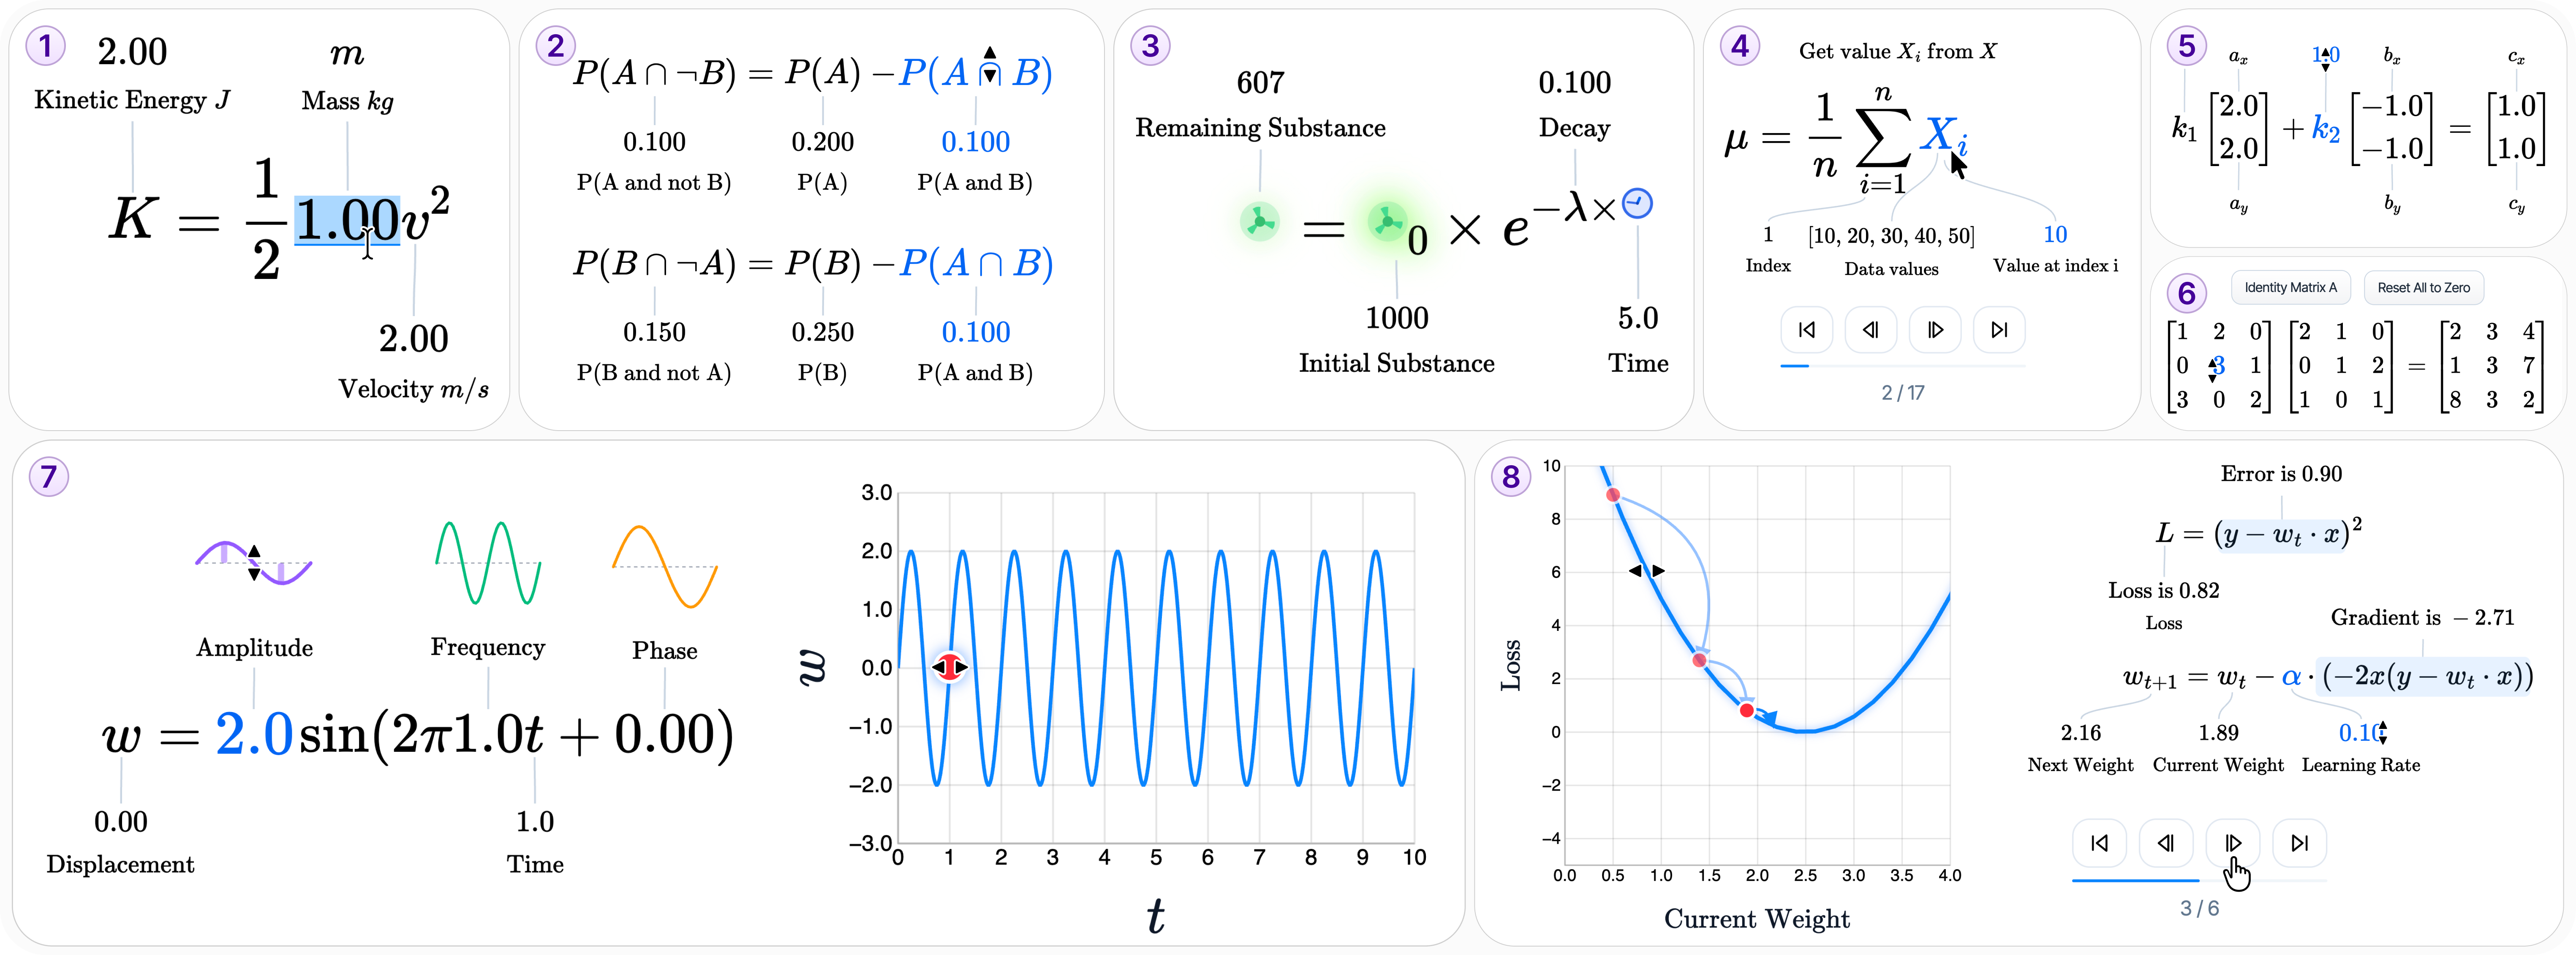
\includegraphics[width=\textwidth]{fig/teaser.png}
  The teaser image goes here.
  \vspace{-1ex}
  \caption{A teaser figure. \normalfont If you are working on a systems paper, you should have a teaser figure here. Teaser figures (1) show the interface in a legible way and (2) need to clearly convey your main conceptual contribution. This is often by cuing up your system on a key use case, and adding appropriate cuing to call out those user interface elements that are central to your conceptual contribution. This caption should express the conceptual contributions in a way that someone could understand even if they didn't read any of the rest of the paper. The style format we tend to use in our captions is first sentence bolded, following sentences unbolded. Usually we add a bit of \texttt{vspace} above and below this caption to make it visually associate more strongly with the image than with the abstract below it.}
  \vspace{2ex}
  \Description{Add your accessibility descriptions to the caption here.}
  \label{fig:teaser}
\end{teaserfigure}

\received[Revised]{29 July 2023}
% \received[revised]{12 March 2009}
% \received[accepted]{5 June 2009}

\maketitle
\ifreview
\raggedbottom
\else
\raggedbottom\pagebreak\flushbottom
\fi
\section{Introduction}\label{intro}

Reading mathematical formulas imposes high cognitive demands: readers must decode symbolic structure, infer relationships between variables, and mentally simulate behavior---imagining how outputs shift as inputs vary or how an algorithm iterates toward a solution~\cite{adams2003reading, Osterholm2006-al}. Interaction can help. Research on learning with multiple representations shows that dynamically linking formulas to visualizations supports comprehension: coordinated representations help learners constrain interpretation and build deeper understanding~\cite{Ainsworth2006-pu}. Direct manipulation can further reduce cognitive effort by closing the gap between a reader's intentions and the system's response, letting users act on mathematical objects and observe outcomes rather than mentally simulating them~\cite{Hutchins1985-wb}.

These findings are reflected in the growing adoption of interactive mathematical content on sites such as Distill.pub and Setosa.io. However, \textit{authoring} these interactions remains prohibitively difficult (Section \ref{FormativeStudy}). Creating a simple interactive formula requires verbose imperative code that entangles computation, state management, interaction logic, and rendering---code that bears no resemblance to the underlying math. To understand this design space, we reviewed 46 interactive formula instances from leading math communication venues including Distill~\cite{distill2017}, Setosa~\cite{setosa2013}, Explorable Explanations~\cite{victor2011explorable}, and others. We found that despite very similar shared types of interactions, nearly all are implemented with custom, case-specific code with no shared abstractions (Section \ref{FormativeStudy}).

Our contribution is \textit{Delta}, a domain-specific language implemented as a React library for authoring interactive mathematical content on the web. Delta is organized around three modes of formula interaction distilled from our analysis of existing interactive explanations: \textit{substitution}, where readers drag symbols directly in a formula and observe how values 
change; \textit{walkthroughs}, where computation \jeff{The introduction of computation here as a thing that happens to formulas is surprising to me. Maybe ``evaluation'' or ``simplification''?} is progressively revealed one step at a time; and \textit{synchronization}, where formula state \jeff{again, ``state'' is not really a thing that formulas have. I think this explanation is mixing ``modes of interaction'' and ``steps to implement interaction''} propagates bidirectionally to linked visualizations. To support these modes, Delta introduces a design that centers on 
five primitives grounded \jeff{$\leftarrow$ What does grounded mean here?}: \textit{formulas} (the \LaTeX{} \jeff{You probably want to say ``notation''?} 
to render), \textit{variables} (which symbols are interactive, their ranges, and display), \textit{semantics} (how values relate computationally), \textit{steps} (how computation is progressively revealed), and \textit{connections} (how formulas synchronize with visualizations). From these primitives, the system derives state management, interactivity, rendering, and synchronized updates. \jeff{I like the punchiness of the preceding two sentences a lot} Beyond the infrastructure, \jeff{own this: ``we also contribute''} an additional contribution is an articulation of what kinds of interactivity should be supported in formulas, distilled from our examples analysis.

We evaluate Delta through two studies. In a controlled comparative study ($n = 19$), participants completed a formula augmentation task faster with Delta than with a baseline React implementation and rated Delta as significantly easier, better suited, and a closer match to how they would describe the task ($p \leq .014$ on all three measures). In an observation study ($n = 10$), participants built interactive formulas from scratch for two mathematical concepts, and we found that Delta's declarative structure is intuitive, scaffolded authoring, and supported pedagogical reasoning. Evaluating the study's data through the framework of the cognitive dimensions of notations, Delta reduced viscosity, diffuseness, and error-proneness \andrew{mismatch between cog dimensions mentioned here and in the results} while exhibiting high closeness of mapping relative to the baseline.

In summary, this paper contributes:
\begin{itemize}
    \item The design and implementation of Delta, a DSL that reifies primitives into a system for authoring where the process of enlivening formulas is made easier and faster.
    \item A system consisting of runtime and React library that supports the authoring of interactive formulas and any linked dynamic representations.
    \item Evidence from usability studies that Delta reduces authoring time and effort compared to a React baseline.
\end{itemize}
\section{Background and Related Work}

In this section, we discuss why authors might wish to augment and enliven mathematical notation paired with dynamic representations, and then situate our system amid related work and tools. 

\subsection{Notation}
 
Mathematic notation is cognitively demanding: readers frequently shift attention between formulas and accompanying prose~\cite{Kohlhase2018-vv}, and readers perform worse on comprehension tasks when a text contains symbols rather than solely prose~\cite{Osterholm2006-al}. As a result, the notation students engage with often requires repeated exposure to understand~\cite{adams2003reading}. Notation has also been reported as an impediment to self-teaching technical topics like machine learning~\cite{Cai2019-lb}.

Subtle changes to the presentation of notation can improve its readability. Coloring and annotating formulas can reduce cognitive load in solving algebra problems~\cite{5c7148d6-681c-3534-885c-7936f89f5133}. Spacing between operators and operands affects how readers interpret order of operations~\cite{Landy2007-zk, Harrison2020-an}. Yet evidence suggest that a static augmentations is still received passively, and deeper understanding requires engagement that goes beyond reading. Chi and Wylie's ICAP framework~\cite{Chi2014-ks} provides empirical support for this intuition, showing that learning deepens as engagement moves from passive reception of information, to active manipulation of materials, to constructive generation of new inferences. A reader who can drag a variable and observe consequences is engaged actively and constructively — activating prior knowledge and inferring relationships. The possibility of deeper learning thus motivates the creation of explorable explanations.

\subsection{Explorable explanations and interactions}

The vision of interactive mathematical content on the web dates back to Bret Victor's ``Explorable Explanations''~\cite{victor2011explorable}, which argued that documents should let readers adjust assumptions and see consequences. Research on learning with multiple representations helps explain why this approach is effective. Ainsworth's DeFT framework~\cite{Ainsworth2006-pu} asserts that multiple representations serve three functions: they \textit{complement} each other, as when a formula supports precise specification while a graph supports perceptual pattern recognition; they \textit{constrain} interpretation, as when concrete visual behavior clarifies abstract symbolic relationships; and they help learners \textit{construct deeper understanding} when integrating across representations promotes abstraction and transfer. 

However, these benefits depend on learners being able to translate between representations---a task research consistently finds difficult. Tools that dynamically link formulas to visualizations could externalize this translation. Hutchins, Hollan, and Norman~\cite{Hutchins1985-wb} provide a cognitive account of how: when an interface lets users manipulate representations as if they were the objects themselves, users experience direct engagement. Interactive formulas aspire to have this quality---the notation becomes the manipulable object itself that could be linked to other representations. Head, Xie, and Hearst~\cite{Head2022-ws} provide the most comprehensive empirical study of formula augmentation practices through a content analysis of 47 documents containing 281 augmented formulas and 1,182 individual augmentations across 16 kinds. Notably, four kinds of interactive augmentations were observed: \textit{scrubbable expressions}, where readers click and drag on a value to change it in place; \textit{editable text fields}, where values can be typed into input boxes; \textit{linked selections}, where hovering over or clicking an expression highlights related content elsewhere in the document; and \textit{external controls}, where input widgets like sliders and drop-down menus outside the formula influence expression values.

To these four categories, the learning sciences suggest a fifth: \textit{formula walkthrough}. The segmenting principle states that learner comprehension improves when complex dynamic content is broken into segments whose advance the learner controls, rather than presented as a continuous sequence~\cite{Plass2009-sq, mayer2001multimedia}. De Jong and van Joolingen (1998) similarly found that gradually introducing complexity produced the strongest gains in learners' intuitive understanding. Dragunov and Herlocker~\cite{Dragunov2003-uy} proposed augmenting formulas with annotations showing how variables are manipulated across derivation stages, and controls that adjust the level of detail in a derivation.

Delta aims to make 5 augmentations - scrubbable expressions, editable text fields, linked selections, external controls, walkthroughs - all achievable with an intuitive grammar design.

\subsection{Tools for augmenting notation}

\paragraph{Markup languages.} LaTeX remains the dominant notation for static mathematical content. On the web, KaTeX~\cite{eisenberg2020katex} and MathJax~\cite{Cervone2012-fd} render LaTeX into high-quality static typeset output, but they are rendering engines that provide no affordances for authoring augmentations. Wu et al.~\cite{Wu2023-xc} introduced FFL, a CSS-like language for \textit{static} formula augmentation. Rather than interleaving styling commands within the LaTeX source, authors write selectors and properties in a companion style specification. FFL's study result showcased how a the separation of augmentation markup from formula markup can reduce viscosity and error proneness compared to a LaTeX baseline. However, FFL is limited to static augmentations. Taking a step towards interactivity, Crichton's Nota~\cite{crichton2021newmedium} and Li et al.'s HeartDown~\cite{Li2022-li} both let authors specify definitions of symbols, with HeartDown going further to make linear algebra papers executable, where editing formula values updates linked figures. While recognizing the importance of linked selections and multiple representations, neither addresses the breadth of basic interactions outlined by Head's empirical study \cite{Head2022-ws}.

\paragraph{Reading interfaces.} Research has explored augmentations that help readers engage with notation in context. Head et al.~\cite{Head2020-eg} designed ScholarPhi, an interface for scientific papers that allows readers to look up symbol definitions in tooltips and equation diagrams overlaid on display equations. Alcock and Wilkinson~\cite{warwick45724} designed e-Proofs, a system for presenting mathematical proofs where readers navigate a sequence of screens that selectively highlight parts of a proof and narrate relationships between lines. Augmented Math~\cite{Chulpongsatorn_2023} and Augmented Physics~\cite{Gunturu_2024} use machine learning and computer vision to retrofit interactive formulas onto static textbook pages. These systems demonstrate the demand for making explorable math notations.

\paragraph{Editing interfaces.} Existing editing interfaces for notation reveal a tension between structure and flexibility. WYSIWYG formula editors such as Microsoft Equation Editor~\cite{microsoft_equation_editor} and MathType~\cite{Topping1999UsingMT} preserve semantic structure but offer no affordances for interactivity. Authors who turn to vector graphics tools like Inkscape~\cite{inkscape} or Google Slides~\cite{google_slides} gain visual flexibility but produce output with no connection to the underlying mathematics --- change a value, and everything must be redrawn by hand. As one author in Head et al.'s study described, ``in Inkscape\ldots{} nothing's attached to anything\ldots{} everything's floating.'' Graspable 
Math~\cite{7821641} shows a third path: by keeping notation semantically grounded, it enables direct manipulation that reflects mathematical meaning, allowing learners to pinch expressions together or drag terms to rearrange equations. Yet its interactions are hardcoded to algebraic laws --- none of these tools let authors specify interactive behavior for their own notation.

\paragraph{Diagramming tools.} Powerful DSLs for mathematical diagramming have displayed a variety of language designs showcasing different strengths. Bluefish~\cite{10.1145/3654777.3676465} is a web-based diagramming framework that replaces React's component model with relations — building blocks like alignment, spacing, and arrows that can share children and specify layout. Grant Sanderson's manim~\cite{manim3b1b} library, as featured in his ~\cite{3blue1brown} video series, can produce rich mathematical animations in Python, and the output is a pre-rendered video. The language is shown to be more lower level in terms of controls, and Head et al.~\cite{Head2022-ws} report that one author estimated it would take a newcomer 1--2 months of use before understanding manim's conceptual model. FigureOne~\cite{figureone2018} is a JavaScript library for drawing, animating, and interacting with shapes, equations, and plots directly in the browser. Its flexible primitives support diagrams, animated equation derivations, and interactive figures. All of these tools feature primitives that are designed around the visual aspect of a mathematic diagram. Delta's design hopes to take a different approach by making use of the semantic and meaning encoded inside the mathematic structure. Adjacent to math, domain-specific primitives in a host language has proven effective in other technical domains. For instance, Hayatpur et al.'s Chisel~\cite{10.1145/3706598.3713723} is a DSL for data structure diagrams, grounded in a content analysis of 80 programmer-produced diagrams. Authors compose diagrams through declarative \textit{abstraction moves} --- selections, revisualizations, simplifications, and annotations --- that incrementally transform a concrete data display into a customized diagram. Another example, Penrose~\cite{10.1145/3386569.3392375}, translates mathematical notation into static diagrams via optimization. Bloom~\cite{Teller2025-pw} extends Penrose into the interactive domain: authors specify optimization constraints, and readers can drag diagram elements while the solver maintains those constraints in real time. Bloom also provides hooks for synchronizing internal diagram state with LaTeX on the page, enabling linked formula–diagram displays. Like Chisel, Delta aims to derives its primitives from an empirical analysis of existing artifacts specific to interactive mathematic explanations. Similar to Penrose, Delta hopes to recognize important semantic items that help govern the resulting artifact.

\subsection{Tools for interactive documents}

Students rely on surrounding prose text for interpretation ~\cite{Shepherd2014-gc} in most math articles. Thus, our work has a dimension of documents and embedding, so we draw on HCI research on interactive document affordances to guide Delta's design.

Existing explorations interactive documents shed light on the importance of \textit{synchronization}, where components are linked to shared states. Tangle.js~\cite{tangle2011} pioneered reactive documents with adjustable numbers: readers drag on numeric values in prose to adjust them, and dependent values update automatically. Inspired by inspired by Tangle.js, Curvenote developed ~\cite{curvenote_components, cockett2024continuous} a similar reactive web-component system. Conlen and Heer's Idyll~\cite{10.1145/3242587.3242600} introduced a reactive document markup language with a component-based architecture. Heer et al.'s Living Papers~\cite{Heer2023-ea} builds on Idyll's AST format to support articles with augmented equations, injecting annotations into KaTeX source and binding event listeners to rendered terms. 

In addition, there is a capability of \textit{substitution} in existing systems where values are substituted into variables in the state and used for computations. For instance, Litt et al.'s Potluck~\cite{potluck2022} demonstrates the broader vision of enriching text documents with reactive computation, by forming a loop of "extract data from text, compute with that data, and then display results back in the text." Similarly, Dragicevic et al.~\cite{10.1145/3290605.3300295} demonstrated ``explorable multiverse analyses,'' where readers can tinker with parameter choices in a research paper and see how results change, illustrating the power of parametric interaction within documents. 

Across all of these systems, a common design gap also emerges: reactivity is decoupled from mathematical structure such that none of the existing systems were able to addresses the basic interactions outlined by  Head's empirical study \cite{Head2022-ws}, to take a step back, none were able to have direct manipulation of formulas as a capability, the rendered formula remains a passive display surface that can be sometimes updated. Delta hopes to extend this space by providing the affordances created by existing systems while making formulas as first-class interactive objects.

\textbf{Computation and visualization platforms.} Several established platforms provide powerful computation and visualization for mathematics. Wolfram Mathematica~\cite{mathematica} offers deep computation and rich visualization, though its browser-based Wolfram Cloud has server-round-trip latency and a subscription requirement. Desmos~\cite{desmos} and GeoGebra~\cite{geogebra} are excellent embeddable tools for graphing and interactive geometry, respectively, but their embedded widgets remain self-contained calculator interfaces with their own sliders and input fields. Formulas within these platforms are not directly manipulable as interactive notation within a surrounding document. 

Across all of the tools surveyed in this section, a common limitation emerges: the rendered formula is not treated as a structured, interactive object. Reactivity operates at the variable-binding layer, entirely separate from the rendered notation. Computation platforms live in their own UI paradigms. None provide direct manipulation of formula symbols or formula-structure-aware interaction. An author who wants a reader to drag a variable in a rendered equation must manually wire overlay elements, event handlers, and state updates — a wide semantic distance, in Hutchins, Hollan, and Norman's~\cite{Hutchins1985-wb} terms, between the intention ("make $\alpha$ draggable") and the specification the system demands. This is exactly the kind of imperative entanglement that Delta seeks to eliminate.
\section{Formative review of artifacts}\label{FormativeStudy}

Head et al.'s prior content analysis~\cite{Head2022-ws} identified four patterns of interactive formula augmentation: scrubbable expressions, editable text fields, linked selections, and external controls. Their focus was on augmentations broadly. Given our focus on interaction, we sought additional documents with this pattern to identify common augmentation forms and better understand potential frictions in their implementation.

We acquired 11 documents containing formulas of interest from sources including Distill.pub, Setosa.io, Explorable Explanations, complex-analysis.com, Georgia Tech's Interactive Linear Algebra textbook, and personal websites. Sources were curated from \citet{Head2022-ws}'s content analysis, \url{https://explorabl.es/}, \url{https://github.com/ubavic/awesome-interactive-math}, and our own web searches. Two authors analyzed 46 formulas of interest. All included formulas were either themselves dynamic or adjacent to and significant in an interactive mathematical explanation.

\paragraph{Augmentation patterns}
Of these, 24 were dynamic (changing following interaction) and 22 supported linking between formula and visualization elements. Formulas were controlled by sliders (8), draggable graph points (17), radio buttons (8), in-formula scrubbing (5), in-formula editing (1). Walkthroughs---step-by-step navigation through staged derivations---appeared for formulas in 1 example and for broader mathematical content in 2 others. We further reviewed the code from open source repositories we found for 11 documents and identified recurring implementation patterns representing potential frictions (see also appendix Table~\ref{tab:formative-audit}):

\begin{itemize}
\item \emph{F1: Diffuseness and tangling (11 articles).} A single interaction is implemented across multiple files; or rendering, layout, and behavior is tangled within a single function.
\item \emph{F2: Indirect identifiers (11 articles).} Variables are referred to in the code using identifiers or array indexing distinct from how the variable appears in the formula.
\item \emph{F3: Fussing the DOM and LaTeX (9 articles)}: The code constructed \LaTeX{} strings programmatically, traversed rendered formula DOM, or both. The two exceptions bypassed LaTeX with their own rendering engines.
\item\emph{F4: Repetition (10 articles)}: interaction logic appeared duplicated across instances of related math objects.
\item\emph{F5: State management (10 articles)}: Articles implemented custom state management and wired up drag handlers, click listeners, and other callbacks to propagate changes across formulas, variables, and other representations.
\end{itemize}

These frictions may distance authors from focusing on presenting a formula well. Our controlled study (Section~\ref{results}) compares Delta to a baseline assess whether improved tooling can reduce this work.
\section{Demo}\label{Demo}

\subsection{Kinetic Energy Example}\label{Kinetic}

\begin{figure*}[t]
  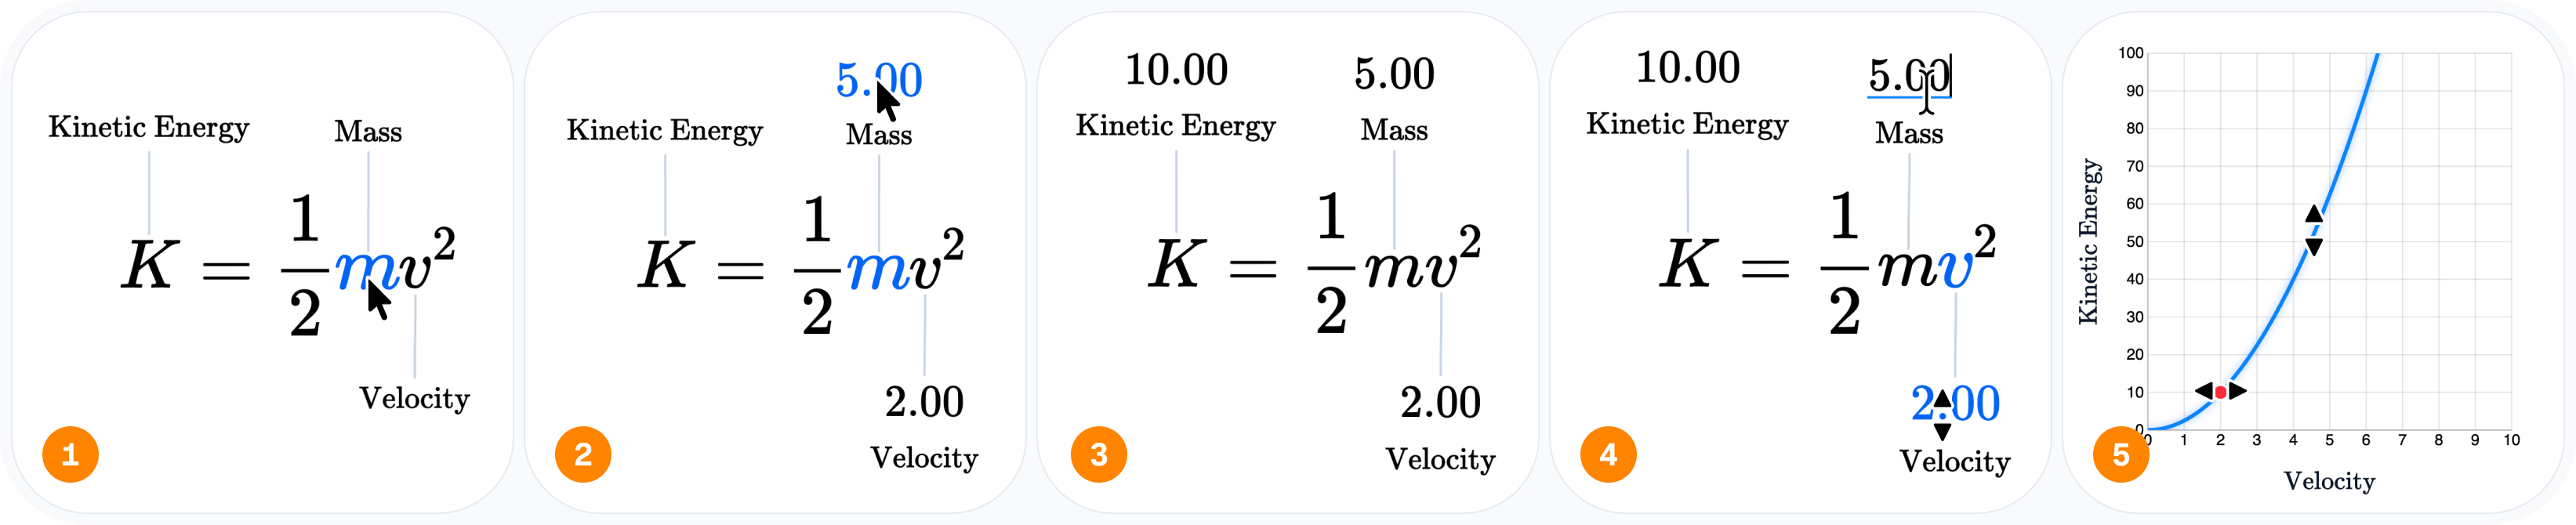
\includegraphics[width=\textwidth]{fig/demo-1.png}
  \caption{Kinetic energy authoring workflow. (1) Declaring variables adds labels. (2) Default values populate them. (3) Semantics compute derived variables. (4) Input modes enable drag and inline editing. (5) A graph entry creates a bidirectional plot.}
  \label{fig:demo-1}
\end{figure*}

Liv is writing a passage about the kinetic energy formula $K = \frac{1}{2}mv^2$. She wants to create an interactive version showing how changes in mass and velocity affect kinetic energy, linked to a synchronized visualization. Instead of writing hundreds of lines of UI code or combining separate math and diagramming packages, Liv imports Delta into her TypeScript file and creates a configuration:

\begin{tcolorbox}[codebox]
\begin{lstlisting}[style=jsstyle]
const kineticConfig: Config = {
  formulas: [
    id: "kinetic-energy", latex: "K = \\frac{1}{2}mv^2",
  ],
  variables: {
    K: { name: "Kinetic Energy" },
    m: { name: "Mass", default: 5 },
    v: { name: "Velocity", default: 2 },
  },
}
\end{lstlisting}
\end{tcolorbox}

To render the formula, Liv places a \texttt{Formula} component inside a \texttt{Provider} that supplies the Delta context:

\begin{tcolorbox}[codebox]
\begin{lstlisting}[style=jsstyle]
<Provider config={kineticConfig}>
  <Formula id="kinetic-energy"/>
</Provider>
\end{lstlisting}
\end{tcolorbox}

In the configuration, each variable key matches the corresponding LaTeX token, so Delta knows which symbol to recognize. Declared variables are visually distinguished with a blue highlight when the reader hovers over their label or symbol (Step~1 in Figure~\ref{fig:demo-1}). Liv adds \texttt{default} values for each variable, which appears in the labels automatically (Step~2 in Figure~\ref{fig:demo-1}). Liv wants $K$ derived from the other variables, so she adds a semantics function. Delta re-executes this function whenever any variable changes, and the $K$ label updates to show the computed value (Step~3 in Figure~\ref{fig:demo-1}):

\begin{tcolorbox}[codebox]
\begin{lstlisting}[style=jsstyle]
semantics: function ({ vars }) {
   vars.K = 0.5 * vars.m * Math.pow(vars.v, 2);
},
\end{lstlisting}
\end{tcolorbox}

To let readers manipulate $m$ and $v$, Liv adds input modes to their variable declarations. Draggable variables show a drag cursor; inline variables can be edited like a text box (Step~4 in Figure~\ref{fig:demo-1}):

\begin{tcolorbox}[codebox]
\begin{lstlisting}[style=jsstyle]
m: { name: "Mass", default: 5, 
     input: "drag", range: [0, 20] },
v: { name: "Velocity", default: 2,
     input: "inline", range: [0, 10] },
\end{lstlisting}
\end{tcolorbox}

Finally, Liv connects the formula to a graph. She adds a \texttt{sample()} call inside her semantics to collect plot coordinates, then declares a \texttt{graph2d} entry. Each line's \texttt{sampleId} links to a \texttt{sample()} call, and \texttt{parameter} specifies the variable Delta sweeps across its range to generate the curve. Interactions on lines and points let readers adjust variable values directly from the plot:

\begin{tcolorbox}[codebox]
\begin{lstlisting}[style=jsstyle]
semantics: function ({ vars, sample }) {
  vars.K = 0.5 * vars.m * Math.pow(vars.v, 2);
  sample("energy", { x: vars.v, y: vars.K });
},
graph2d: [{
  id: "energy-graph",
  xAxisVar: "v", yAxisVar: "K",
  lines: [{
    sampleId: "energy", parameter: "v",
    interaction: ["vertical-drag", "m"],
  }],
  points: [{
    sampleId: "energy",
    interaction: ["horizontal-drag", "v"],
  }],
}],
\end{lstlisting}
\end{tcolorbox}

Liv renders the graph with \texttt{<Graph id="energy-graph"/>} inside the \texttt{Provider}. She now has a formula--graph pair that allows bidirectional manipulation: dragging the curve changes $m$, and dragging the point changes $v$, with both the formula labels and graph updating in lockstep (Step~5 in Figure~\ref{fig:demo-1}).

\subsection{Average Example}\label{Average}

\begin{figure*}[t]
  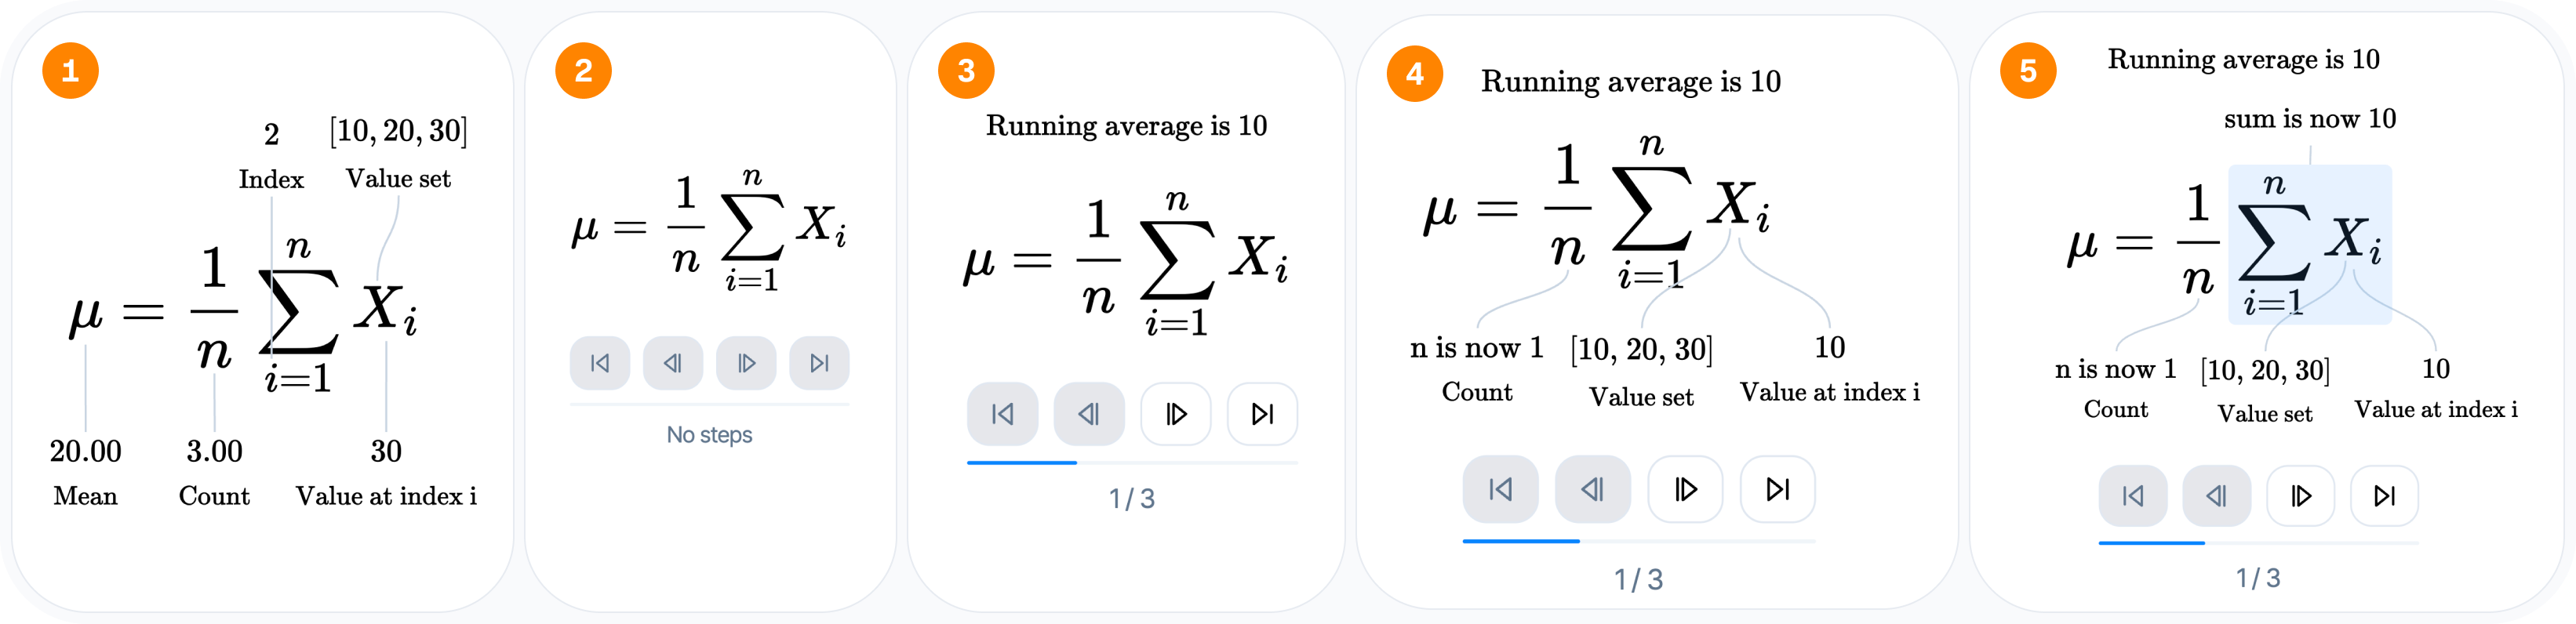
\includegraphics[width=\textwidth]{fig/demo-2.png}
  \caption{Average walkthrough authoring workflow. (1) Semantics produce final labels. (2) Stepping mode adds controls. (3) \texttt{step()} calls define pause points. (4) Labels anchor values to symbols. (5) LaTeX expression keys highlight notation spans.}
  \label{fig:demo-2}
\end{figure*}

Liv is now writing about the average formula $\mu = \frac{1}{n} \sum_{i=1}^{n} X_i$. She wants to walk students through the computation, showing how the running average evolves as each value is incorporated. She declares her formula and variables---including an array-valued variable \texttt{X}---and writes a semantics function that loops over the array:

\begin{tcolorbox}[codebox]
\begin{lstlisting}[style=jsstyle]
const config: Config = {
  formulas: [{
    id: "average",
    latex: "\\mu = \\frac{1}{n} \\sum_{i=1}^{n} X_i",
  }],
  variables: {
    "\\mu": { name: "Mean" },
    n: { name: "Count" },
    i: { name: "Index", precision: 0 },
    X_i: { name: "Value at index i", precision: 0 },
    X: { default: [10, 20, 30], name: "Value set" },
  },
  semantics: function ({ vars }) {
    vars.n = vars.X.length;
    var sum = 0;
    vars["\\mu"] = 0;
    for (var i = 0; i < vars.n; i++) {
      vars.i = i;
      vars.X_i = vars.X[i];
      sum = sum + vars.X_i;
      vars["\\mu"] = sum / (i + 1);
    }
    vars["\\mu"] = Math.round(vars["\\mu"] * 100) / 100;
  },
}
\end{lstlisting}
\end{tcolorbox}

With this configuration, the formula renders with labels showing the final computed values (Step~1 in Figure~\ref{fig:demo-2}). However, the loop executes all at once---the reader only sees the end result. To let students follow the computation one iteration at a time, Liv sets \texttt{stepping: true} and inserts \texttt{step()} calls inside the loop body. Each call marks a pause point and accepts a \texttt{description} and a \texttt{labels} object:

\begin{tcolorbox}[codebox]
\begin{lstlisting}[style=jsstyle]
stepping: true,
semantics: function ({ vars, step }) {
  ...
  for (var i = 0; i < vars.n; i++) {
    ...
    vars["\\mu"] = sum / (i + 1);
    step({
      description: "Running average is " + vars["\\mu"],
      labels: {
        "\\sum_{i=1}^{n} X_i": "sum is now " + sum,
        n: "n is now " + (i + 1),
        X_i: vars.X_i,
        X: vars.X,
      },
    });
  }
  vars["\\mu"] = Math.round(vars["\\mu"] * 100) / 100;
},
\end{lstlisting}
\end{tcolorbox}

With stepping enabled, Delta presents navigation controls (Step~2 in Figure~\ref{fig:demo-2}) rendered via a \texttt{StepControl} component. If \texttt{step()} calls are added in the semantics, by clicking forward, the display updates according to the step. (Step~3 in Figure~\ref{fig:demo-2}). Each key in the \texttt{labels} object is either a variable identifier or a LaTeX expression from the formula. Variable keys display values as labels beneath their symbol (Step~4 in Figure~\ref{fig:demo-2}); LaTeX expression keys highlight the corresponding notation span and attach the label to it (Step~5 in Figure~\ref{fig:demo-2}). At the first step, the summation span highlights with ``sum is now 10,'' $n$ shows ``n is now 1,'' and $X_i$ displays 10.  Students can trace the full trajectory of the running average, seeing how each new value shifts the mean, all without leaving the formula.
\section{System}\label{System}

Delta is a DSL implemented as a React library for augmenting mathematical formulas and surrounding explanations with interactivity. Authors write a configuration that declares formulas as \LaTeX{} strings---the notation authors already know---variables as interactive symbols, a semantics function for computation, and visualizations that synchronize with the formula state. A \texttt{Provider} component abstracts away all MathJax setup and reactive update logic (Table~\ref{tab:mathjax-comparison}); authors place \texttt{Formula} and \texttt{Graph} components by \texttt{id} alongside prose and other content. Common interactive patterns require minimal configuration beyond the formula itself, while the specification is compositional---each addition extends what came before, so authors moving beyond defaults build on existing work rather than starting over.

\subsection{Substitution}

\paragraph{Input.} Delta supports the four interaction patterns identified by Head et al.~\cite{Head2022-ws} through three input mechanisms. \textit{In-formula input}: within the rendered formula, \texttt{drag} variables enable scrubbable expressions where readers click and drag on a value to change it in place, while \texttt{inline} variables replace symbols with editable text fields for direct entry. \textit{In-prose input}: \texttt{InlineVariable} components place the same draggable or editable controls within running text, functioning as external controls that influence formula values from outside the expression. \textit{Custom input}: authors create arbitrary input widgets---sliders, dropdowns, or domain-specific controls---via \texttt{Custom()} components that read and write values through the \texttt{vars} proxy (Table~\ref{tab:custom-api}). Linked selections emerge automatically: hovering over any variable highlights it across all \texttt{Formula}, \texttt{InlineVariable}, and \texttt{Custom} components sharing that identifier. A compact set of properties---\texttt{input}, \texttt{range}, \texttt{step}, \texttt{default}, \texttt{name}---allows rapid specification of essential presentation dimensions (Table~\ref{tab:variable-properties}). In a gradient descent walkthrough (Figure~\ref{fig:system}), an \texttt{InlineVariable} in the prose lets readers drag the label $y$---and dragging directly on the graph updates $y$ just the same.

\paragraph{Computation.} The \texttt{semantics} function provides expressiveness in computation: authors access variables by the same identifiers used in the formula---\texttt{vars.x} reads or writes \texttt{x}---then write plain JavaScript with full access to loops, conditionals, external libraries, and helper functions for complex calculations (Table~\ref{tab:vars-access}). When any input changes, Delta automatically re-executes the semantics function. Because the same function handles \texttt{step()} calls for walkthroughs and \texttt{sample()} calls for visualizations, a single computation pass updates all dependent data.

\subsection{Walkthroughs}

Delta supports walkthroughs that \textit{align sequencing with semantics}: the narrative structure of an explanation maps directly onto the computational structure of the formula. Within the semantics function, authors insert \texttt{step()} calls at meaningful points in the computation---after computing a gradient, before updating a weight---breaking the algorithm into discrete, narrated stages that mirror how the math actually unfolds. When \texttt{stepping: true} is set, the system presents navigation controls for stepping forward and backward, letting readers trace the same logical path the computation follows. This proves especially valuable for iterative algorithms like gradient descent, where each pass through the loop updates multiple interdependent quantities that readers must track together.

Each \texttt{step()} accepts a configuration object with two properties: \texttt{description} for narrated annotations and \texttt{labels} for positioning values on the formula. Descriptions support inline \LaTeX{} with \texttt{\$...\$} and string concatenation with computed variables from the semantics function---e.g., \texttt{`Error is \$\{vars.error\}\$`}---so annotations stay synchronized with the current state. Labels use \LaTeX{} substrings as selectors: keys matching variable identifiers (e.g., \texttt{w\_t}) attach values to those symbols, while keys matching longer expressions (e.g., \texttt{y - w\_t \textbackslash cdot x}) highlight and annotate entire subexpressions. This selector syntax leverages authors' existing \LaTeX{} knowledge---the same strings that define the formula also address its parts. Label values can be numbers, strings with inline \LaTeX{}, or formatting calls such as \texttt{latex()}, \texttt{precision()}, and \texttt{sigfig()} that mirror the display settings available on variables themselves (Table~\ref{tab:variable-properties}).

The gradient descent walkthrough (Figure~\ref{fig:system}) illustrates these constructs working together across multiple formulas. In the loss formula, labels display the current error value on the squared-error expression; in the update rule, separate labels show the gradient, current weight, and next weight at their respective positions. Because \texttt{step()} accepts a record keyed by formula \texttt{id}, authors specify which labels appear on which formula at each stage---the loss computation shows its intermediate values while the weight update shows its own, all advancing in lockstep as readers navigate the walkthrough.

\subsection{Synchronization}\label{Visualizations}

\paragraph{Variables.} A core principle underlies the system: \textit{variables are universal indices}. The same \LaTeX{} token that appears in the formula serves as the key that connects notation, interactivity, computation, and visualization under a single identifier. As a result, variables are defined apart from formulas in Delta. Separating variables from formulas also enables multi-formula systems driven by a single semantics function, reduces reliance on symbolic solvers, and gives authors flexibility to design custom computational flows. The same \texttt{vars} interface is used not just in \texttt{semantics}, but also in custom components.

\paragraph{Synchronized representations.} Delta synchronizes formulas with visualizations so that manipulating one representation updates the other, keeping formula and graph as synchronized representations of the same object. A \texttt{Provider} component abstracts away all MathJax setup and reactive update logic (Table~\ref{tab:mathjax-comparison}); authors place \texttt{Formula} and \texttt{Graph} components by \texttt{id} alongside prose and other content.

\paragraph{Sampling.} To populate a plot, the semantics function emits data with \texttt{sample(sampleId, \{x, y\})} or \texttt{sample(sampleId, \{x, y, z\})}, separating the mathematical relationship from sampling and rendering. In 2D, \texttt{lines} sample over a parameter variable's range via \texttt{parameter}, while \texttt{points} display the current state; both reference data through \texttt{sampleId}. The \texttt{interaction} property enables bidirectional manipulation---e.g., \texttt{interaction: ["horizontal-drag", "x"]} lets readers drag a point to change \texttt{x}. Points and vectors can also synchronize with step-through mode via \texttt{stepId}, optionally accumulating across steps with \texttt{persistence: true}. 3D plots extend the same model to surfaces and meshes, rendered with Plotly.js. Users can also access the same programmatic sampling helpers directly---\texttt{sample2DLine()}, \texttt{sample2DPoint()}, \texttt{sample3DLine()}, \texttt{sample3DPoint()}, and \texttt{sampleSurface()}---and Delta uses these same calls internally to implement the library's \texttt{Graph} component. The \texttt{graph2d} and \texttt{graph3d} arrays declare plots that react to formula state; because variables serve as universal indices, the same identifiers key both semantics and visualization data.

\paragraph{useStore.} For domain-specific needs, authors can register custom React components via \texttt{Custom()}, which injects a \texttt{vars} proxy for reading and writing variable values while preserving the reactive connection. Lower-level components can also access the surrounding reactive state through \texttt{useStore()}, the hook used by Delta's built-in components to read and write variables within the enclosing \texttt{Provider}. The \texttt{Graph} component renders a visualization by \texttt{id}, composing freely alongside \texttt{Formula} and other content.

\begin{figure*}[t]
\centering
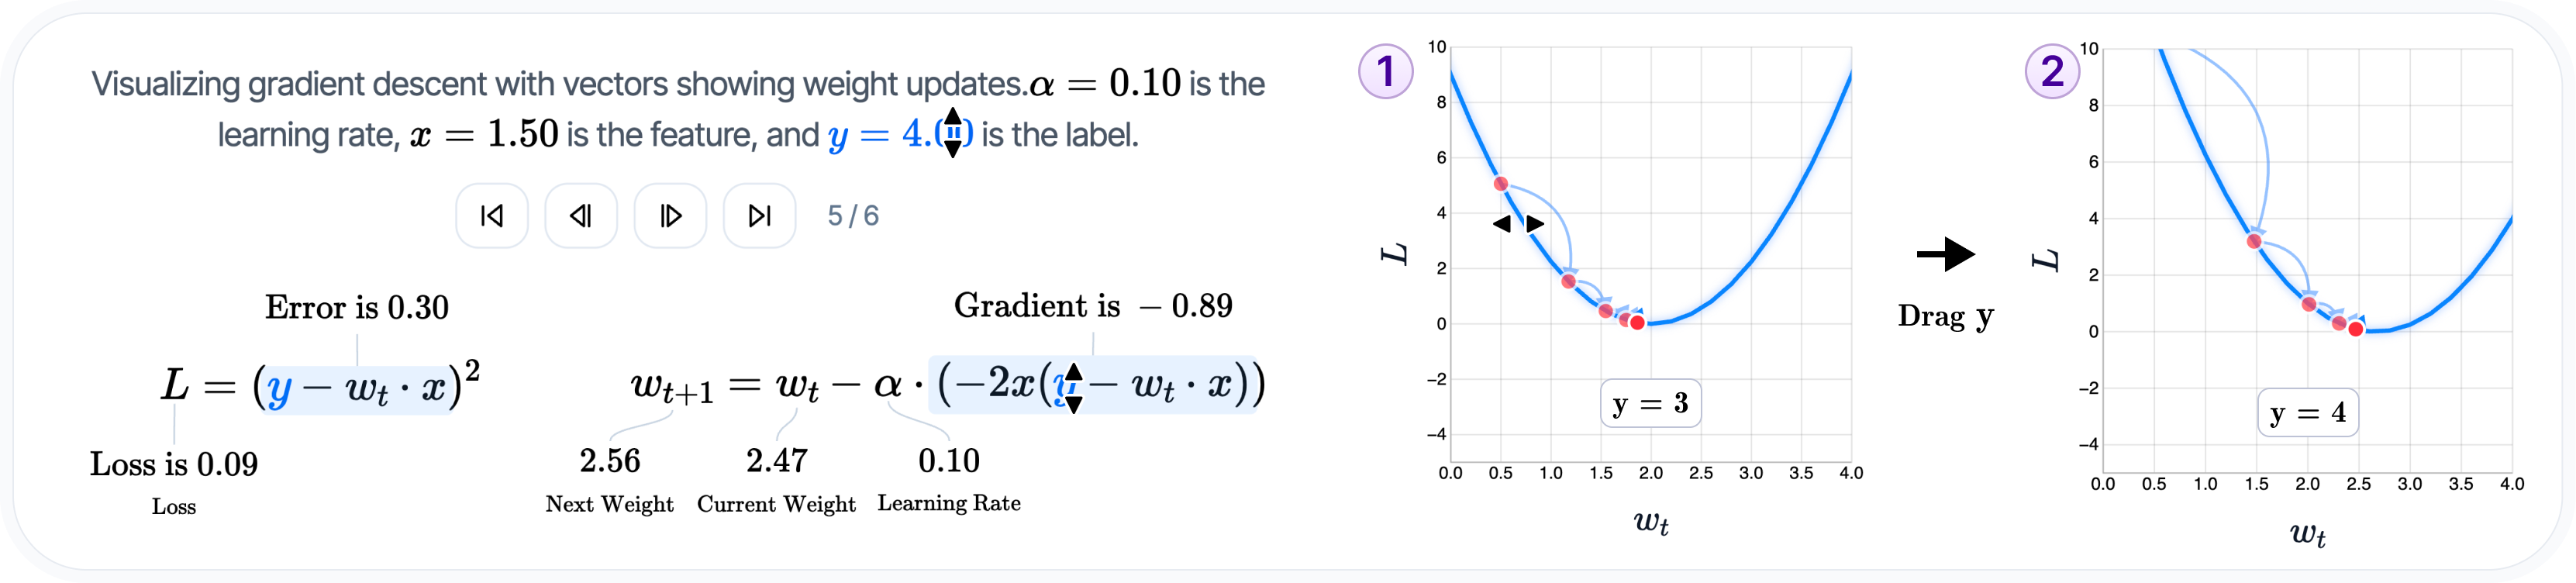
\includegraphics[width=\textwidth]{fig/system.png}
\caption{\textbf{Reactive propagation across steps and visualizations.} Dragging $y$ in the prose (1) triggers re-execution of the semantics function, updating all intermediate step values and shifting the visualization vectors (2) to reflect the new loss landscape. See Figure~\ref{fig:gradient-config} for the full configuration.}
\label{fig:system}
\end{figure*}

\section{Implementation}

Delta is a JSON DSL with an accompanying React component library that propagates state across components. One of the intents is of Delta is to take care of common logistical aspects of making formulas interactive so that authors can instead focus on presentation. We describe those aspects here. 

\paragraph{Parsing and rendering}
Delta parses and augments formulas in a manner largely consistent with other recent formula augmentation tools~\cite{Wu2023-xc,tao2025freeform}. It leverages the parser from KaTeX~\cite{tool:katex}, a widely-used LaTeX web formula renderer, to produce an AST of a formula's LaTeX. On this AST, it matches specified variables and then wraps them with macros that will wrap those variables in CSS IDs at render time. If a spec asks to replace a variable with the value, Delta replaces the variable node with a value node. Delta serializes the parse tree into LaTeX and then passes it to MathJax to render it to HTML. A re-parse and re-render of the formula is invoked whenever the contents change, i.e., whenever a substituted value is updated. Labels are rendered as elements on a ReactFlow canvas and spaced using a custom collision resolution algorithm.

\paragraph{Interaction handling}
After MathJax renders the augmented LaTeX into the DOM, Delta attaches interaction handlers to the identified elements using synthesized CSS IDs from the earlier step. To promote continuity of interactions, event handlers are attached to transparent overlay nodes positioned over each variable. This prevents disruption of interaction as the formula changes, for instance if concrete values are substituted into the formula and are changing in response to interaction.

\paragraph{Data collection and updates}
To support the gamut of interactions, state is saved in a shared store, comprising current values of all variables, status of which variables are hovered, and steps and samples saved from executing the semantics function. Delta uses MobX, a reactive state management library, to coordinate updates across the system. When a change is triggered in variable value, MobX triggers re-execution of the semantics function and then re-rendering of any affected formula components. Other components---such as inline variables embedded in prose and custom components---access values through React Context and are wrapped with MobX's \texttt{observer} to re-render automatically when values change.
\section{Controlled Study}\label{results}
To evaluate Delta's impact on the experience of authoring augmentations, we conducted a remote comparative usability study. The study was designed to answer the following questions:

\vspace{0.5em}
\noindent\textbf{RQ1.} Does Delta reduce the time to augment an existing interactive formula compared to a baseline React approach?
\\
\noindent\textbf{RQ2.} Does Delta reduce the effort to augment an existing interactive formula compared to a baseline React approach?
\vspace{0.5em}

\subsection{Methodology}

\paragraph{Participants} We recruited 19 graduate students and upper division undergraduates from a private university's engineering school, across computer science, data science, computer graphics, and robotics. Our target users are potential authors of interactive math web documents — a role without a well-defined professional category. Since such authors likely combine mathematical typesetting fluency with web development skills, we operationalized eligibility around three competencies - \LaTeX{} formulas, JavaScript, and basic React, verified through a screening survey. Participants rated their comfort writing \LaTeX{} formulas as a median of 4 on a 5-point Likert scale ($\sigma = 0.91$); 11 wrote \LaTeX{} weekly, 5 monthly, and 3 less than monthly. They rated their comfort writing JavaScript as a median of 4 ($\sigma = 1.12$); 9 wrote JS weekly, 8 monthly, 1 daily, and 1 less than monthly. Regarding React experience, 6 had professional experience, 6 had personal or academic experience, and 7 had limited personal or academic experience\andrew{how limited? so limited we shouldn't take them as representative users?}. We refer to these participants by anonymized random double-digit numeric identifiers (e.g., P21, P48).

\paragraph{Setup} Study sessions took place remotely over Zoom and were recorded. Participants used their own computers to retain familiar input configurations, and logged into GitHub in Google Chrome using their personal accounts. Each task had a dedicated branch in a GitHub Codespace — an online IDE — pre-loaded with template code. Survey data was collected via Google Forms within the same browser session.

\paragraph{Tasks} The task exercised the core aspects distinguishing Delta's config-based structure from a baseline React approach: variable declaration, interaction configuration, labels, and derived computation. Participants were given a starter implementation of an interactive formula for kinetic energy ($K = \frac{1}{2}mv^2$), where $K$ and $v$ were already interactive---dragging $v$ updated the computed value of $K$---but $m$ was static. Participants were asked to make $m$ draggable (with values ranging from 0 to 10 in increments of 1, defaulting to 1), add a label displaying its current value and description, and ensure $K$ updated correctly based on both $m$ and $v$. A reference video demonstrated the target behavior. Participants were given 20 minutes per task, a limit determined through informal pilot testing \andrew{why was it chosen to be 20?}. 

The study was within-subjects: each participant completed the task with both libraries in sequence. Library order was counterbalanced (9 baseline-first, 10 Delta-first) to mitigate learning effects.\andrew{within-subjects pretty unconventional for programming studies (usually learning effects are massive), will have to justify why learning effects don't undermine results here} Instead of a demonstration or practice session, participants received written API tutorial materials they could reference freely throughout.\andrew{why on-demand references instead of practice session?}

\paragraph{Baseline} We compared Delta to a baseline React implementation where authors manually manage React state, annotate LaTeX strings with \texttt{\textbackslash cssId\{\}} references, and wire up components with matching props for hover, drag, and display. This represents the conventional approach, where interactivity is assembled imperatively from low-level primitives rather than declared in a configuration. Both conditions began from examples with identical appearance interactive behavior, allowing us to observe viscosity\andrew{first time this term appears} in a controlled manner. Since Delta provides formula-rendering UI components, we moved the baseline's UI component code into separate, non-editable files to minimize confounding factors---particularly diffuseness and cognitive load from UI boilerplate.\andrew{not totally sure what you are saying here\ldots{} I think it is something about reducing confounds due to poor organization of React starter code by hiding away as much unnecessary complexity as possible} This allowed participants in both conditions to avoid navigating unrelated infrastructure. The resulting editable file was 61 lines in the baseline and 40 lines in Delta.

\paragraph{Measures.} We collected behavioral measures from screen recordings and subjective measures from post-task questionnaires. Behavioral measures included \textit{completion time}, \textit{guide reading time}, \textit{number of guide views}, and \textit{notes on irrelevant edits}.\andrew{why were these captured, what were you hoping to determine using them?} Participants could indicate when they believed they were finished; completion time was measured from first edit to researcher verification that all requirements were met, with participants asked to continue if any were unmet. Those who exceeded the 20-minute limit were stopped and their time recorded as 20 minutes. For subjective measures, participants completed a questionnaire after both conditions. On a 7-point Likert scale (1 = baseline, 4 = about the same, 7 = Delta), they rated which library was (1) easier to complete the task with, (2) better suited for the task, and (3) a better match for the language they would use to describe the task. Participants also provided free-text explanations for each rating.

\paragraph{Analysis.} Because our data are paired and not assumed to be normally distributed, we use the Wilcoxon signed-rank test for all behavioral comparisons. For subjective Likert ratings, we test whether responses differ significantly from the neutral midpoint (4) using a one-sample Wilcoxon signed-rank test. We report Cohen's $d$ for paired samples as a measure of effect size where applicable.

\subsection{Results}

\paragraph{Effect on task speed (RQ1).}
Nearly all tasks (37 of 38, 97\%) were completed within the 20-minute time limit. All 19 tasks done with Delta were completed within the limit; one participant (P30) did not finish with the baseline. Participants completed the task significantly faster with Delta ($\text{Mdn} = 5.4$ min, $\text{M} = 5.3$ min, $\text{SD} = 1.8$ min) than with the baseline ($\text{Mdn} = 9.4$ min, $\text{M} = 10.5$ min, $\text{SD} = 4.4$ min); Wilcoxon $W = 6.0$, $p < .001$, Cohen's $d = 1.16$. Of 19 participants, 16 were faster with Delta. The median speedup was $1.87\times$.\andrew{checking --- to me this implies (1) computing speedup individually for all participants; (2) sorting list of speedups; (3) picking middle value. if that's not what this is, may need another phrase}

We observed a significant order effect on the magnitude of the time difference between conditions (Mann-Whitney $U = 88.0$, $p < .001$). Participants who used the baseline first showed a larger advantage for Delta (mean difference $= 8.9$ min) than those who used Delta first (mean difference $= 1.8$ min). This suggests that task familiarity compressed completion times in the second condition regardless of library. Critically, even within the more conservative subgroup that used Delta \textit{first}, Delta was still significantly faster (Wilcoxon $W = 6.0$, $p = .027$, $n = 10$), with 7 of 10 participants completing the task faster with Delta.

\begin{figure}[H]
  \centering
  \framedfig{fig/completion_time.pdf}
  \caption{Task completion times by tool. Delta led to significantly faster completion times than the baselines regardless of order effects.}
  \label{fig:completion_time}
\end{figure}

Six of 19 participants (32\%) attempted edits in irrelevant parts of
the codebase with the baseline, compared to only 1 (5\%) with Delta.
\andrew{how was this measured?}
Three participants resorted to using browser developer tools to
inspect element with the baseline; none did so with Delta.

\paragraph{Subjective ratings.}
Participants rated Delta significantly above the neutral midpoint on all three scales: ease ($\text{Mdn} = 7$, $\text{M} = 6.42$; $W = 1.5$, $p < .001$), suitability ($\text{Mdn} = 6$, $\text{M} = 5.84$; $W = 9.0$, $p = .001$), and language match ($\text{Mdn} = 7$, $\text{M} = 5.53$; $W = 26.5$, $p = .014$). Eighteen of 19 participants rated Delta as easier (scores of 5--7); the one exception was P30, who valued the baseline's proximity to idiomatic React (``Library A felt easier to understand'').\andrew{what were the levels for the baseline?}

\begin{figure}[H]
  \centering
  \framedfig{fig/subjective_ratings.pdf}
  \caption{\textbf{Post-task subjective ratings.} Participants rated which library was easier, better suited, and a better language match on a 7-point scale (1\,=\,Baseline, 4\,=\,Same, 7\,=\,Delta; $n = 19$). All 3 measures favored Delta significantly ($p \leq .014$).}
  \label{fig:subjective_ratings}
\end{figure}

\paragraph{Qualitative findings.}
Participants' free-text responses revealed qualitative differences in \textit{where} each tool imposed cognitive load. 

The most frequently cited pain point with the baseline was the \texttt{\textbackslash cssId\{\}} mechanism---manually annotating LaTeX strings with CSS identifiers and ensuring they match across component props. Seven participants (P11, P14, P20, P79, P87, P88, P99) reported confusion or errors with this step (e.g., P88: ``I forgot to add the cssId on the LaTeX element `m'\,''; P87: ``Felt a little clunky using \texttt{\textbackslash\textbackslash cssId}''). More broadly, seven participants (P45, P55, P79, P80, P87, P88, P99) described the baseline as requiring edits across multiple disconnected locations---state declarations, component props, and the LaTeX string---even within the abstracted file (P55: ``making the small change to make m modifiable with a drag motion required changes in several parts of the code''). 

By contrast, 14 of 19 participants reported no confusion or difficulty with Delta, attributing this to co-located variable configuration: all properties for a given variable were specified in a single place (P48: ``Less places to adjust code''; P80: ``all I had to do was add a few lines of code that were very similar to the existing code''). Several participants (P11, P20, P45, P57, P79, P80) noted that Delta's structure matched their mental model of the task---P45 observed it let them ``place all the requirements in one config, using the same language as described by the task.''\andrew{this will not be seen as particularly compelling --- we controlled the language of the task, so it might be seen as obvious that it would reflect how we designed the language} The most common Delta error was forgetting to update the \texttt{semantics} function after adding a new
variable (P11, P17, P19, P50, P55, P87), a mistake participants quickly self-corrected once the computed value did not update.

Two participants (P29, P14) preferred the baseline on suitability
and language dimensions despite completing the task faster with
Delta. Both cited familiarity with React idioms: P14, among the
most experienced React developers in the sample, felt the baseline
``gave me more control,'' and P29 noted it ``works more seamlessly
with the rest of a React app''---pointing to a tension between
task-specific efficiency and integration with existing workflows.
\section{Observation Study}\label{observational}

Our first study assessed a comparison to a baseline on a simple task; our second study sought to assess tasks that were less constrained and more complex. We asked participants to build up two kinds of augmentations where they had freedom in the precise outcome. We sought to understand (1) if could they learn enough of Delta to succeed (2) the appropriateness of the various language constructs.

\subsection{Methods}

\paragraph{Participants.}
Ten of the 19 participants from the controlled study (Section \ref{results}) took part in an observation study. We sampled in this way for convenience; we already knew these participants could pass our inclusion criteria. A consequence of this choice is that participants already had some small amount of training in Delta. In aggregate, participant backgrounds was very similar to the prior study: participants rated their comfort writing LaTeX formulas as a median of 4 on a 5-point Likert scale ($\sigma = 1.03$) and with JavaScript as a median of 3.5 ($\sigma = 1.43$). All had some prior experience with React. Below, we refer to participants by anonymized identifiers assigned to them during the study (e.g., P21, P48).

\paragraph{Setup.} Like the controlled study, these study sessions were held on Zoom with coding taking place in a GitHub Codespace.

\paragraph{Tasks.}

Each participant completed two open-ended formula authoring tasks, each lasting up to 30 minutes. In each task, participants were given an empty Delta config as a starting point, with placeholders for formulas, variables, and semantics. They were given a task sheet that provided the formula's LaTeX, background about the formula, an example scenario with concrete values, and questions that could motivate potential augmentation ideas. Participants were instructed to augment the formula in whatever way they thought best helped a reader understand the underlying concept; the task sheets stated ``there is no single right answer'' and encouraged participants to try alternatives. Task~2 additionally required that the augmentation include at least one step.

Tasks were chosen to test essential parts of the Delta language. Task 1 (T1) assessed the basic interaction and notation features, while Task 2 (T2) evaluated the stepping syntax. Graphing and SVG features were excluded to keep session length feasible (already ${\sim}$2 hours); they depended on features from T1 and T2, so we prioritized those features instead.
T1 required augmentation of a formula for radioactive decay formula $N(t) = N_0 \cdot e^{-\lambda t}$ and T2 a formula for expected value $E = \sum_{x \in X} x\, P(x)$. Prior to each task, participants followed a self-paced written tutorial introducing all features they might need for the task on an example formula. They were given 20 minutes.

% \vspace{0.5em}
% \noindent
% \fbox{\begin{minipage}[t]{0.44\columnwidth}
% \centering
% \textbf{T1:} \textit{Radioactive decay}
% \[N(t) = N_0 \cdot e^{-\lambda t}\]
% \end{minipage}}%
% \hfill
% \fbox{\begin{minipage}[t]{0.44\columnwidth}
% \centering
% \textbf{T2:} \textit{Expected value}
% \[E = \sum_{x \in X} x\, P(x)\]
% \end{minipage}}
% \vspace{0.5em}

% \noindent
% Both tasks provided starter code with imports in place and asked participants to fill in a Delta configuration---specifying formulas, variables, and semantics---to make the formula interactive. participants were given the relevant LaTeX as a starting point and were encouraged to augment the formula in whatever way they thought best helped a reader understand the underlying concept. Each task sheet included background on the formula, an example scenario with concrete values, and suggested questions for exploration.

% \vspace{0.5em}
% \noindent
% \fbox{\begin{minipage}[t]{0.44\columnwidth}
% \centering
% \textbf{T1:} \textit{Radioactive decay}
% \[N(t) = N_0 \cdot e^{-\lambda t}\]
% \end{minipage}}%
% \hfill
% \fbox{\begin{minipage}[t]{0.44\columnwidth}
% \centering
% \textbf{T2:} \textit{Expected value}
% \[E = \sum_{x \in X} x\, P(x)\]
% \end{minipage}}
% \vspace{0.5em}


\paragraph{Duration.}
Each task lasted up to 30 minutes, after which the facilitator stopped the author. Although tasks were open-ended with no fixed completion criteria, all ten participants produced a working interactive formula with correct computation and semantics and had time to iterate on its design. Including tutorials, questionnaires, and transitions, sessions lasted approximately 2 hours.

\paragraph{Measurement and Analysis.}
9 of 10 sessions were facilitated by the same researcher; 1 by a second researcher following the same protocol. Participants were told to think aloud, and the facilitator could interrupt with process questions. Post-task questionnaires after each task asked participants to rate usefulness, intuitiveness, and difficulty of Delta's main features on Likert scales and elaborate in free text. Because each task introduced different features, questionnaires asked only about features relevant to that task---basic interaction and notation for T1, stepping for T2. Both researchers independently reviewed recordings and compiled timestamped observation logs documenting feature usage patterns, error sequences, recovery strategies, and notable utterances. One researcher then performed qualitative coding across all data, identifying common workflows, design successes, and gaps. Retained codes were those lending insight into designing future DSLs like Delta.

\subsection{Results}

All ten participants completed both tasks within the allotted 30 minutes each.
% We report self-reported intuitiveness and difficulty ratings from the post-task questionnaires alongside qualitative observations from the think-aloud sessions. Figure~\ref{fig:obs-intuitiveness} summarizes the intuitiveness Likert-scale ratings for both tasks. Self-reported difficulty ratings followed a largely similar distribution and are included in the appendix (Figure~\ref{fig:obs-difficulty}).
We first describe design successes and then gaps. Design successes are organized using the Cognitive Dimensions of Notations framework~\cite{Blackwell2003-gv}, which provides a vocabulary for evaluating the usability of notational systems like DSLs. We foreground two dimensions that were central concerns in our design process: \emph{closeness of mapping} (how naturally the notation maps to the problem domain) and \emph{viscosity} (effort to make small changes).

\begin{figure}[t]
  \centering
  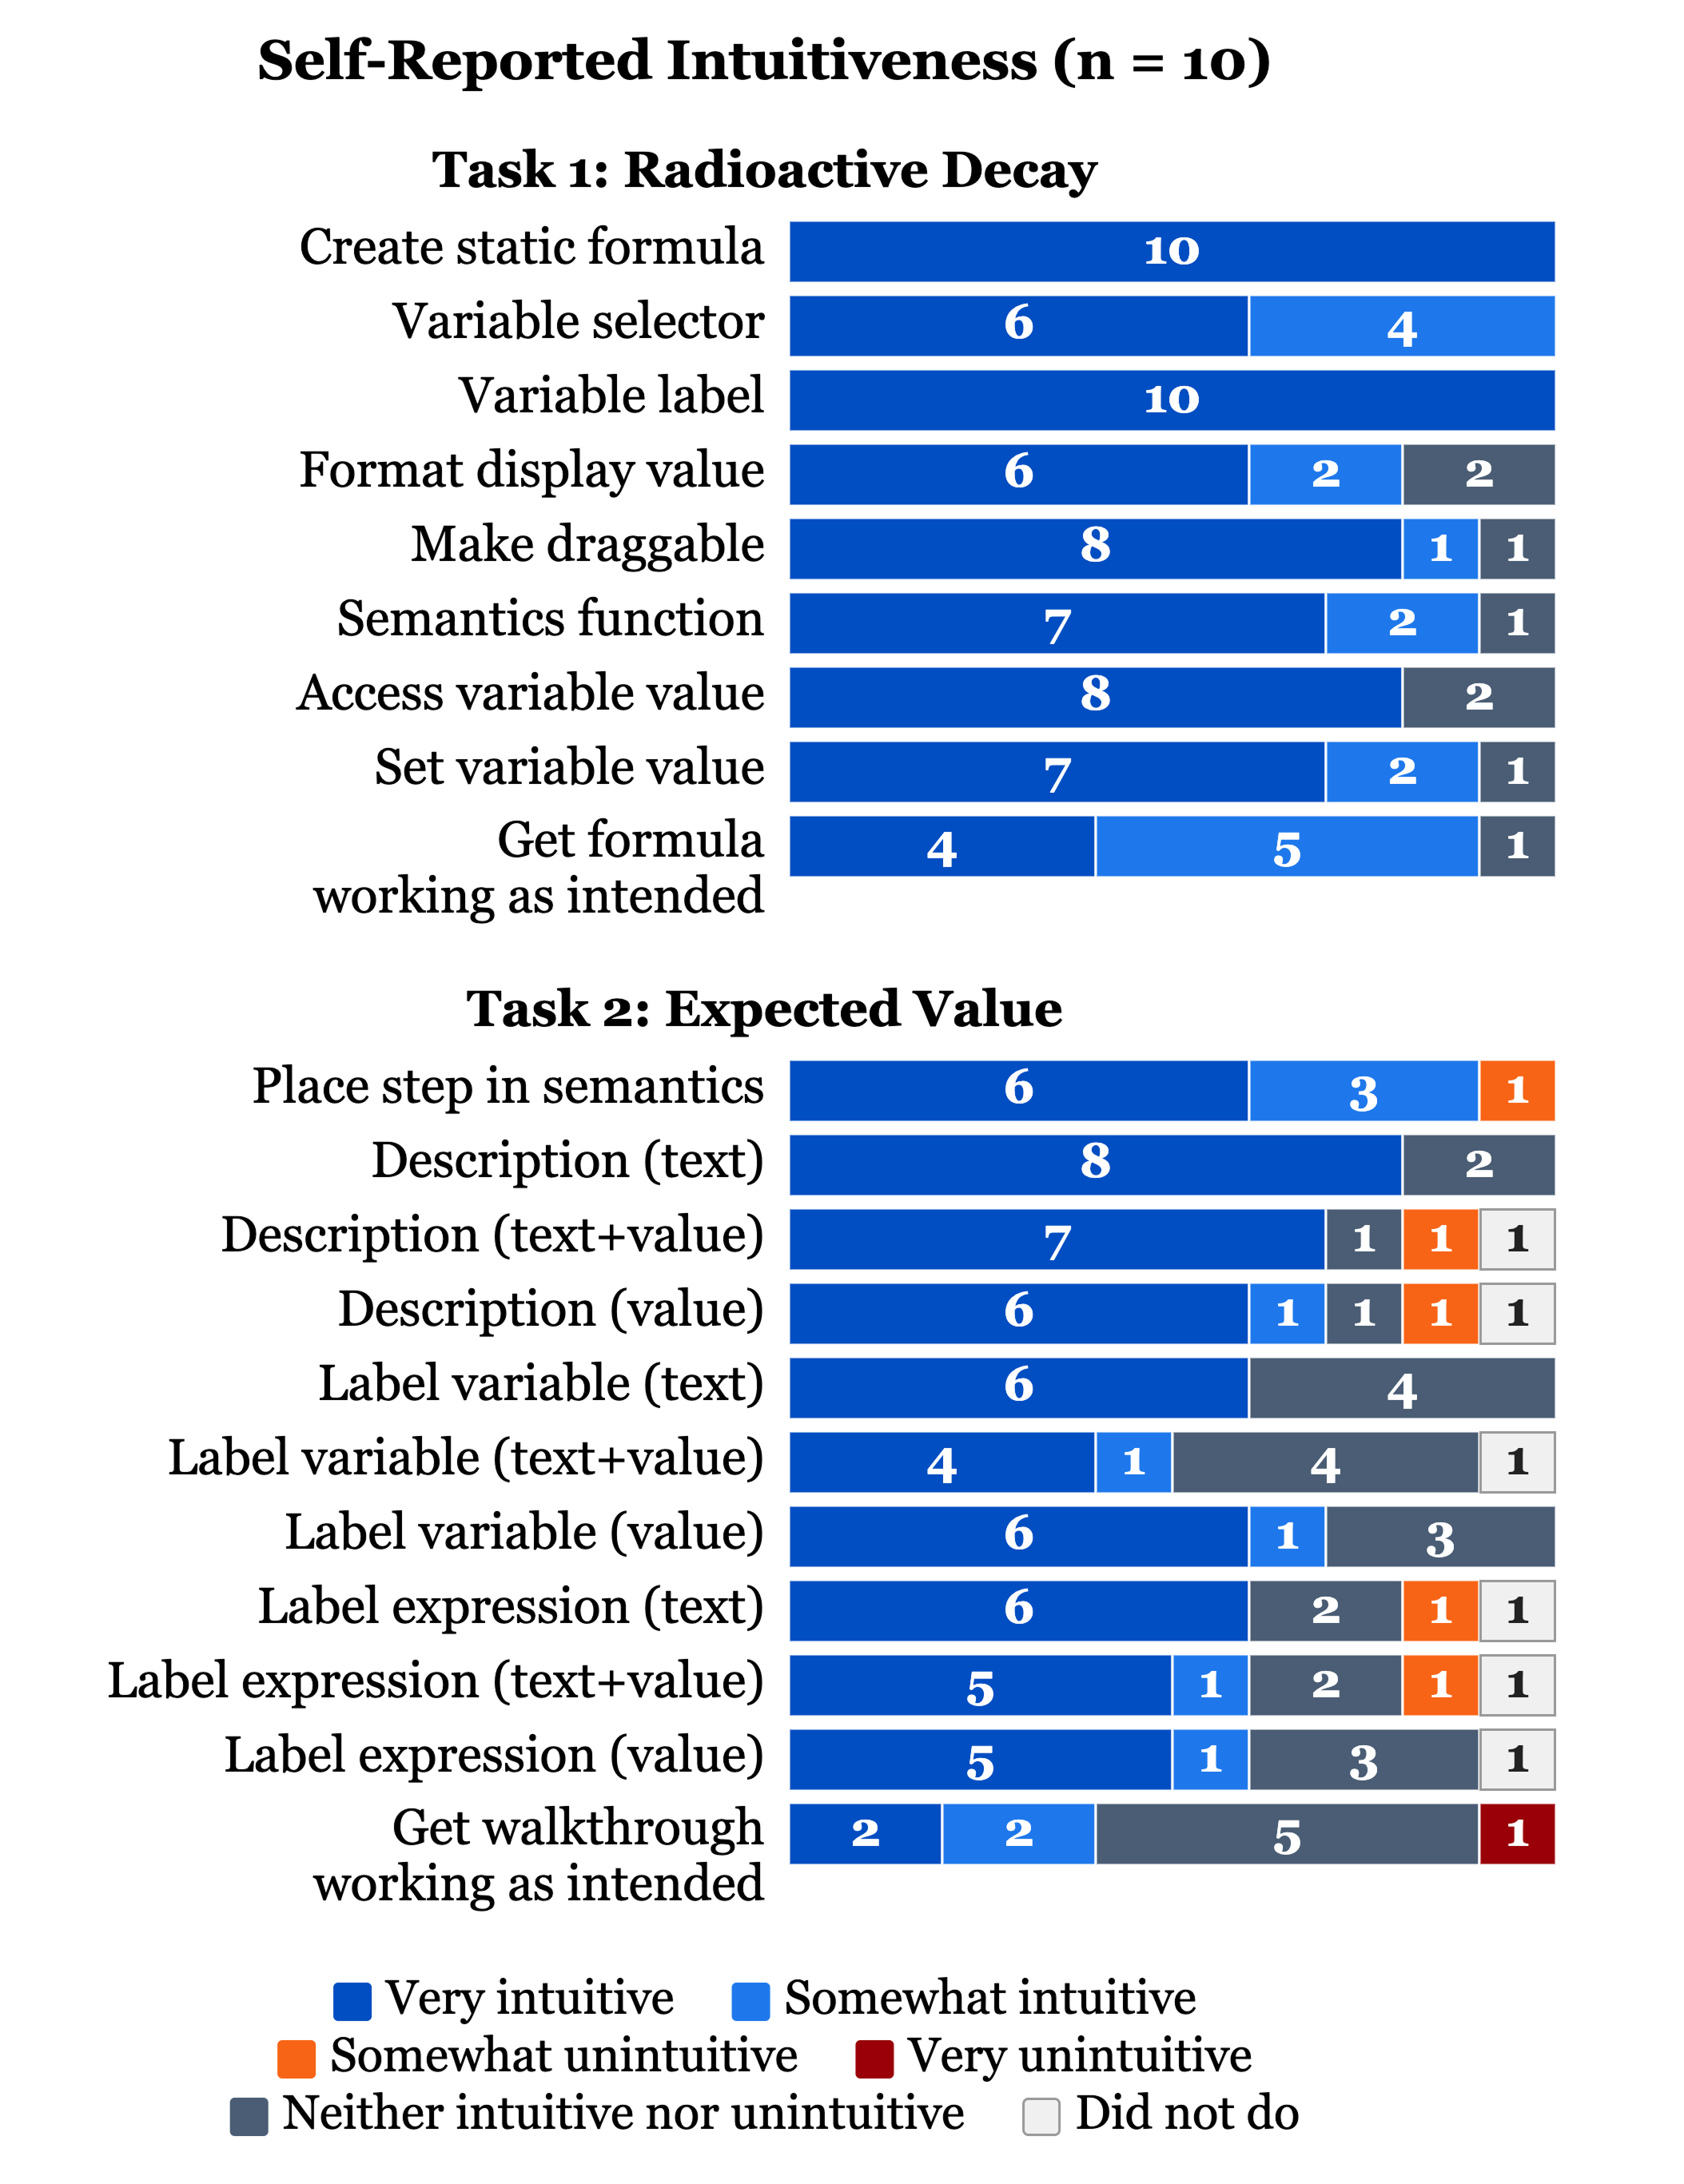
\includegraphics[width=\columnwidth]{fig/intuitiveness.png}
  \caption{\textbf{Self-reported intuitiveness ratings.} participants rated the intuitiveness of library features on a 5-point Likert scale ($n = 10$). Task~1 covers nine basic interaction and notation features; Task~2 covers eleven stepping features.}
  \Description{Diverging stacked bar chart showing Likert-scale intuitiveness responses for both tasks side by side. Most bars are dominated by blue (very intuitive / somewhat intuitive), with more spread visible for holistic items like getting the formula or walkthrough working as desired.}
  \label{fig:obs-intuitiveness}
\end{figure}

\subsubsection{Closeness of mapping}
All participants reported intuitiveness and difficulty of all language constructs and overall process for both tasks. Construct intuitiveness was our proxy for closeness of mapping; distributions of ratings appear in in Figure~\ref{fig:obs-intuitiveness}; difficult followed similar distributions and is in the appendix (Figure~\ref{fig:obs-difficulty}). Nearly all features were rated majority ``very'' or ``somewhat intuitive,'' with basic features (from T1) appearing particularly intuitive. Below, we single out particular features here that were the sites of interesting behavior and participant commentary.

\medskip

% We report self-reported intuitiveness and difficulty ratings from the post-task questionnaires alongside qualitative observations from the think-aloud sessions. Figure~\ref{fig:obs-intuitiveness} summarizes the intuitiveness Likert-scale ratings for both tasks. Self-reported difficulty ratings followed a largely similar distribution and are included in the appendix (Figure~\ref{fig:obs-difficulty}).

\emph{Variables as IDs.} Our language uses LaTeX variable strings as indexes into the formula and calculation state. This seemed to work well, with 6 participants describing it ``very intuitive'' and 4 ``somewhat.'' Participants named variable IDs capably; 6 were able to reference complex variables like ``$N(t)$ and ``$\lambda$'' correctly on their first try, and 7 were able to select expressions in walkthrough steps correctly on their first try.

\emph{Computation.} The semantics function---plain JavaScript---was well received: accessing variable values was rated ``very intuitive'' by 8 of 10 participants, and expressing computation by 7 of 10. It seems that for some participants the control flow of semantics transferred well to structuring walkthroughs, with \texttt{for} loops for summations (P57: ``Oh, I have to use a for loop---they all need to do the same thing''), \texttt{if} statements for case logic (P45), and local variables for readability (9 of 10 participants). P48 noted ``placing steps [is] pretty intuitive because [it] follows how your brain thinks about math expressions,'' and P57 observed ``once the template of the formula was setup, writing the steps was fast.''

\emph{Walkthrough labels}
Delta's formatting utilities for walkthrough labels---\texttt{sigFigs}, \texttt{precision}, and \texttt{latex()}---were adopted successfully on first use as 7 participants refined their displays. 3 participants \texttt{latex()} with \texttt{sigfigs()} or \texttt{precision()} to format step labels on their first attempts.

\medskip

One further piece of evidence of the constructs' appropriateness was that participants reached for them driven by higher-level intent about how best to present the formula.
Several participants (P48, P11, P19, P17, P29) paused to reason about pedagogical effectiveness. In T1, P48 concluded that ``some questions relate to how much time has passed,'' making time interactive. P19 chose not to make $\lambda$ draggable, reasoning ``lambda is a constant.'' P11 reasoned about physical constraints: ``Time should never be negative. Let's have a range for that.'' P29 said ``For the first step I can define a set of possible values X and on the second step I can decompose the sum.''

\subsubsection{Viscosity}
Delta was designed to let authors build up formulas one bit at a time, from static formula to gradual addition and refinement of augmentations. We saw participants take advantage of this possibility. 8 of 10 participants regularly alternated between editing code and checking rendered output. 4 reviewed a static formula before declaring any variables; 3 initialized empty variable declarations and verified their correctness by highlighting them through by hovering over the formula; and 3 assigned and rendered labels before doubling back to define semantics and interactivity. Across both tasks, formatting of labels tended to follow a two-phase pattern: 8 of 10 participants first focused on getting computation correct---defining variables, writing semantics, and verifying values---before returning to adjust presentation with significant figures, precision, or LaTeX rendering. 5 participants demonstrated or expressed that the language allowed them to localize edits, modifying one aspect of the specification without ripple effects across others. Participants largely followed the default configuration structure---first providing LaTeX, then variables, then semantics (8 of 10 participants); the alternative was writing out the semantics first (P57, P19). 

\subsubsection{Gaps}\label{design-gaps} 

We saw two recurring gaps. The first was trouble selecting the right instance of a variable when it appeared multiple times in a formula (5 participants). This problem has a syntactical solution in FFL~\cite{Wu2023-xc} which could be ported to Delta. The second gap is that  stepping requires setting a modal flag. 3 participants got stuck when they forgot to set the flag. One solution could be to enable stepping by default as soon steps are added to semantics.
\section{Discussion}

\subsection{Limitations}

\paragraph{Task scope and ecological validity.}
Both studies used a single task type---augmenting or authoring an interactive formula---within a controlled IDE environment. Real-world authoring involves longer sessions, larger codebases, and integration with surrounding prose, visualizations, and build systems, where Delta's advantages on viscosity and diffuseness may interact with factors we did not measure.

\paragraph{Participant population.}
Our participant pool, while appropriate for the target user profile, consisted of graduate and advanced undergraduate students at a single institution. Professional content authors or domain experts with different tool fluencies may experience Delta differently.

\paragraph{Order effects.}
The controlled study's within-subjects design introduced a significant order effect: task familiarity compressed second-condition times regardless of library. Although Delta remained significantly faster even in the conservative Delta-first subgroup, the magnitude of the overall speedup ($1.87\times$) likely overstates what would be observed in a between-subjects design.

\paragraph{Implementation gaps.}
Delta's current lack of disambiguation for repeated symbols (G1) and the multi-step activation required for stepping (G2) introduced avoidable friction in the observation study. Resolving these would likely shift both behavioral and subjective measures further in Delta's favor.

\subsection{Future Work}

\paragraph{Direct manipulation of structured mathematical objects.}
The design gaps around array-valued variables (G3) and repeated-symbol disambiguation (G1) raise a broader question: how should a DSL expose mechanisms for readers to interactively modify variables declared as vectors, matrices, or indexed sets? Answering this requires both new interaction techniques and formal models of how symbolic structure maps to manipulable regions---a problem that connects formula authoring to the wider HCI literature on structured editors and direct manipulation~\cite{hutchins1985direct}.

\paragraph{Graphical authoring interfaces.}
Delta's configuration structure is sufficiently declarative that it could serve as the backing model for higher-level authoring interfaces. Because the specification cleanly separates variable declarations, interaction settings, and semantics, a graphical editor could let non-programmers author interactive formulas without writing code. Such an interface would lower the entry barrier beyond what a text-based DSL alone can achieve and open questions about how to design direct-manipulation editors for domain-specific languages.
 
\paragraph{AI-assisted authoring.}
The pedagogical reasoning we observed---authors deliberating over which variables to make interactive, what ranges are physically meaningful, and how to sequence steps---suggests that Delta's primitives could serve as a foundation for intelligent authoring support. A system that infers plausible variable ranges from domain knowledge or suggests step decompositions from a formula's algebraic structure would shift the authoring bottleneck from implementation to pedagogical design.

\paragraph{Variable-conditional semantics and solver-like interaction.}
Delta currently re-executes a single semantics function whenever any variable changes, treating all updates uniformly. A natural extension is to allow authors to specify \textit{which} computation runs in response to \textit{which} variable changing. Under such a model, dragging one variable could solve for another. Designing an authoring abstraction that remains declarative while exposing per-variable semantic dispatch poses an open DSL design challenge.
\section{Conclusion}

We presented Delta, a domain-specific language whose declarative primitives reify the recurring patterns we identified across 46 existing interactive formula instances into a coherent authoring model. In two user studies, Delta made formula augmentation faster and easier than a conventional React approach, and in open-ended tasks its declarative structure scaffolded not only implementation but also pedagogical reasoning about what to make interactive and why. More broadly, Delta demonstrates that a well-chosen set of domain-specific abstractions can collapse the distance between mathematical intent and interactive artifact — a principle likely to generalize to other domains where authors want to make formal notation explorable. We hope this work opens new lines of inquiry into DSL-driven authoring tools, graphical interfaces built atop declarative specifications, and intelligent support that shifts the bottleneck from implementation to pedagogical design.

\begin{acks}
Spend a bit of time reflecting on all of the people from the HCI community, at our institution and others, who have given you feedback and input on this work.
If anyone has given you feedback that has been useful to you, we should acknowledge them here.
If there were an subject matter experts or user representatives who participated in your formative research pro bono, thank them here (though generally don't name them unless we have their permission).
Thank anyone else who paid us a big favor who is not on the author list, like someone who created a video figure for this paper, ran study sessions, or gave exceptional feedback on a paper draft.
Ask Andrew who we have to thank for funding.
If you are on fellowship, we should acknowledge that fellowship here.
\end{acks}

\bibliographystyle{ACM-Reference-Format}
\bibliography{refs,andrew-base,andrew-extras}

\appendix
\clearpage

\section{Delta Configuration Grammar}

\noindent\begin{minipage}{\textwidth}
  \small
  \begin{align*}
  \langle \textit{Config} \rangle &::= \{ \; \texttt{formulas}: \langle \textit{Formulas} \rangle, \;
      \texttt{variables}: \langle \textit{Vars} \rangle, \;
      \texttt{semantics}: \langle \textit{Sem} \rangle, \\
      &\quad\;\; [\texttt{graph2d}: \langle \textit{G2D} \rangle^*], \;
      [\texttt{graph3d}: \langle \textit{G3D} \rangle^*], \\
      &\quad\;\; [\texttt{stepping}: \textit{bool}], \; \} \\[3pt]
  %
  \langle \textit{Formulas} \rangle &::= [\langle \textit{Formula} \rangle^+] \qquad
  \langle \textit{Formula} \rangle ::= \{ \; \texttt{id}: \textit{str}, \; \texttt{latex}: \textit{str} \; \} \\[3pt]
  %
  \langle \textit{Vars} \rangle &::= \{ \; (\textit{sel} : \textit{num} \mid \langle \textit{VarSpec} \rangle)^* \; \} \\
  \langle \textit{VarSpec} \rangle &::= \{ \; [\texttt{name}: \textit{str}], \;
      [\texttt{default}: \textit{num}], \;
      [\texttt{input}: \texttt{"drag"} \mid \texttt{"inline"}], \\
      &\quad\;\; [\texttt{range}: [\textit{min}, \textit{max}]], \;
      [\texttt{step}], \; [\texttt{precision}], \; [\texttt{sigFigs}], \\
      &\quad\;\; [\texttt{latexDisplay}: \langle \textit{Disp} \rangle], \;
      [\texttt{labelDisplay}: \langle \textit{Disp} \rangle], \\
      &\quad\;\; [\texttt{svgContent}: \langle \textit{SVGFn} \rangle], \;
      [\texttt{svgSize}: \{w,h\}] \; \} \\
  \langle \textit{Disp} \rangle &::= \texttt{"name"} \mid \texttt{"value"} \mid \texttt{"svg"} \mid \texttt{"none"} \\[3pt]
  %
  \langle \textit{Sem} \rangle &::= \texttt{function} \; (\{ \texttt{vars}, \texttt{sample}, \texttt{step}, \texttt{latex} \}) \; \langle \textit{Body} \rangle \\
  \langle \textit{Body} \rangle &::= \{ \; \langle \textit{Stmt} \rangle^* \; \} \\
  \langle \textit{Stmt} \rangle &::= \texttt{vars.}\textit{id} \; \texttt{=} \; \langle \textit{Expr} \rangle \;\mid\;
      \texttt{sample}(\textit{id}, \{ \texttt{x}, \texttt{y}, [\texttt{z}] \}) \\
      &\mid \texttt{step}(\langle \textit{StepSpec} \rangle, [\textit{blockId}]) \;\mid\;
      \texttt{latex}(\textit{n}).\texttt{precision}(\textit{d}) \;\mid\; \langle \textit{JSStmt} \rangle \\
  \langle \textit{StepSpec} \rangle &::= \{ \; [\texttt{description}: \textit{str}], \;
      [\texttt{labels}: \{ (\textit{sel}: \textit{val})^* \}] \; \} \\[3pt]
  %
  \langle \textit{G2D} \rangle &::= \{ \; \texttt{id}: \textit{str}, \;
      [\texttt{xAxisLabel}], \; [\texttt{yAxisLabel}], \;
      [\texttt{xRange}], \; [\texttt{yRange}], \\
      &\quad\;\; [\texttt{lines}: \langle \textit{Line2D} \rangle^*], \;
      [\texttt{points}: \langle \textit{Pt2D} \rangle^*], \;
      [\texttt{vectors}: \langle \textit{Vec} \rangle^*] \; \} \\[3pt]
  %
  \langle \textit{Line2D} \rangle &::= \{ \; \texttt{sampleId}: \textit{str}, \;
      \texttt{parameter}: \textit{sel}, \;
      [\texttt{range}], \; [\texttt{samples}], \;
      [\texttt{interaction}: \langle \textit{Drag} \rangle] \; \} \\
  \langle \textit{Pt2D} \rangle &::= \{ \; \texttt{sampleId}: \textit{str}, \;
      [\texttt{interaction}: \langle \textit{Drag} \rangle], \;
      [\texttt{stepId}], \;
      [\texttt{persistence}] \; \} \\
  \langle \textit{Vec} \rangle &::= \{ \; \texttt{startSampleId}: \textit{str}, \;
      \texttt{endSampleId}: \textit{str}, \;
      [\texttt{label}], \\
      &\quad\;\; [\texttt{interaction}: [\textit{xVar}, \textit{yVar}]], \;
      [\texttt{curved}], \;
      [\texttt{stepId}], \;
      [\texttt{persistence}] \; \} \\
  \langle \textit{Drag} \rangle &::= [\texttt{"horizontal-drag"} \mid \texttt{"vertical-drag"}, \textit{varId}] \\[3pt]
  %
  \langle \textit{G3D} \rangle &::= \{ \; \texttt{id}: \textit{str}, \;
      [\texttt{xRange}], \; [\texttt{yRange}], \; [\texttt{zRange}], \\
      &\quad\;\; [\texttt{surfaces}: \langle \textit{Surf3D} \rangle^*], \;
      [\texttt{lines}: \langle \textit{Line3D} \rangle^*], \;
      [\texttt{points}: \langle \textit{Pt3D} \rangle^*] \; \} \\
  \langle \textit{Surf3D} \rangle &::= \{ \; \texttt{sampleId}: \textit{str}, \;
      \texttt{parameters}: [\textit{v}_1, \textit{v}_2], \;
      [\texttt{ranges}], \; [\texttt{samples}], \; \} \\
  \langle \textit{Line3D} \rangle &::= \{ \; \texttt{sampleId}: \textit{str}, \;
      \texttt{parameter}: \textit{sel}, \;
      [\texttt{range}], \; [\texttt{samples}] \; \} \\
  \langle \textit{Pt3D} \rangle &::= \{ \; \texttt{sampleId}: \textit{str}, \; \}
  \end{align*}
  \captionof{figure}{\textbf{Grammar for Delta configuration language.} \textmd{Styling properties (e.g., \texttt{color}, \texttt{fontSize}, \texttt{labelFontSize}, \texttt{lineWidth}, \texttt{opacity}) and the React component library are omitted. A \textit{sel} (selector) is a LaTeX token (e.g., \texttt{"v"}, \texttt{"\textbackslash\textbackslash mu"}) identifying a variable. Abbreviations: \textit{str}=string, \textit{num}=number, \textit{bool}=boolean. $\langle \textit{Expr} \rangle$ and $\langle \textit{JSStmt} \rangle$ are JavaScript expressions/statements. $\langle \textit{SVGFn} \rangle$ receives the current variable's value and all other variables (\texttt{environment}) from the runtime, returning an SVG string for dynamic variable icons. Square brackets denote optional fields.}}
  \label{fig:bnf-grammar}
  \end{minipage}

\clearpage

\section{Patterns in code from formative analysis}

\begin{minipage}{\textwidth}
\centering
\begin{tabular}{@{}llccccc@{}}
\toprule
\textbf{Article} & \textbf{Source} & \textbf{F1} & \textbf{F2} & \textbf{F3} & \textbf{F4} & \textbf{F5} \\
\midrule
Backprop Explainer            & Individual developer    & $\bullet$ & $\bullet$ & $\bullet$ & $\bullet$ & $\bullet$ \\
Traveling Wave -- Sine Waves  & FigureOne               & $\bullet$ & $\circ$   & $\bullet$ & $\bullet$ & $\bullet$ \\
OLS Regression                & Setosa.io               & $\bullet$ & $\bullet$ & $\bullet$ & $\bullet$ & $\bullet$ \\
Eigenvectors \& Eigenvalues   & Setosa.io               & $\bullet$ & $\bullet$ & $\bullet$ & $\bullet$ & $\bullet$ \\
Why Momentum Really Works     & Distill.pub             & $\bullet$ & $\bullet$ & $\bullet$ & $\bullet$ & $\bullet$ \\
Understanding GNNs            & Distill.pub             & $\bullet$ & $\bullet$ & $\bullet$ & $\bullet$ & $\bullet$ \\
ILA: Least Squares            & Georgia Tech            & $\bullet$ & $\bullet$ & $\bullet$ & $\bullet$ & $\bullet$ \\
ILA: Systems of Equations     & Georgia Tech            & $\bullet$ & $\bullet$ & $\bullet$ & $\bullet$ & $\bullet$ \\
ILA: Vectors                  & Georgia Tech            & $\bullet$ & $\bullet$ & $\bullet$ & $\bullet$ & $\bullet$ \\
Roots of Complex Numbers      & complex-analysis.com    & $\bullet$ & $\circ$   & $\circ$   & $\circ$   & $\bullet$ \\
The Complex Power Function    & complex-analysis.com    & $\bullet$ & $\bullet$ & $\bullet$ & $\bullet$ & $\bullet$ \\
\midrule
\textbf{Total}                &                         & \textbf{11/11} & \textbf{9/11} & \textbf{10/11} & \textbf{10/11} & \textbf{11/11} \\
\bottomrule
\end{tabular}
\captionof{table}{Formative study thematic coding results. \textmd{Each cell indicates whether the pattern was observed ($\bullet$) or not ($\circ$) in the article's source repository. Codes for frictions: \textbf{F1}~Diffuseness and tangling, \textbf{F2}~Indirect identifiers, \textbf{F3}~Fussing the DOM and LaTeX, \textbf{F4}~Repetition, \textbf{F5}~State management. See Section~\ref{FormativeStudy} for definitions.}}
\label{tab:formative-audit}
\end{minipage}

\clearpage

\section{Examples from formative analysis}

\begin{minipage}{\textwidth}
\centering
\begin{minipage}[t]{0.48\textwidth}
\begin{lstlisting}[basicstyle=\ttfamily\scriptsize, frame=single, title={\texttt{fig2.js:123--139} (amplitude control)}]
let offset = 0.5;
mover.notifications.add('setTransform', () => {
  offset += mover.getPosition().y * 2;
  mover.transform.updateTranslation([0, 0]);
  if (offset > 1) { offset = 1; }
  if (offset < -1) { offset = -1; }
  const newA = offset * 2;
  trace.update(sine(newA));
  eqn.updateElementText({
    A: `${Math.abs(newA).toFixed(1)}`,
    sign
  });
});
\end{lstlisting}
\end{minipage}
\hfill
\begin{minipage}[t]{0.48\textwidth}
\begin{lstlisting}[basicstyle=\ttfamily\scriptsize, frame=single, title={\texttt{fig3.js:129--142} (wavelength control)}]
let offset = 0;
mover.notifications.add('setTransform', () => {
  offset += mover.getPosition().x;
  mover.transform.updateTranslation([0, 0.15]);
  if (offset > 1) { offset = 1; }
  if (offset < -1) { offset = -1; }
  const newR = offset * 3 + 5;
  trace.update(sine(newR));
  eqn.updateElementText({
    value: `${newR.toFixed(1)}`
  });
});
\end{lstlisting}
\end{minipage}
\captionof{figure}{\textbf{Schema duplication in the Traveling Wave article~\cite{FigureOne-TravelingWave}.} \textmd{Two figures implement the same interaction schema---a draggable parameter controlling a sine wave---with structurally identical code. Both blocks maintain local \texttt{offset} state, accumulate drag input, clamp to bounds, transform to a parameter value, update the trace, and refresh the equation label. The only differences are which axis is read (\texttt{.y} vs \texttt{.x}), which parameter is computed (\texttt{newA} vs \texttt{newR}), and which label field is updated. This pattern, where the same mathematical interaction schema is copy-pasted and lightly edited per instance, appeared in 10 of 11 audited articles.}}
\label{fig:schema-duplication}
\end{minipage}

\begin{minipage}{\textwidth}
\centering
\begin{minipage}[t]{0.48\textwidth}
\begin{lstlisting}[basicstyle=\ttfamily\scriptsize, frame=single, title={OLS Regression: DOM geometry for highlight positioning}]
// After render, measure tspan elements
var svgBB = this.getDOMNode().getBoundingClientRect();
var beta1Text = this.refs.beta1Text.getDOMNode();
var beta1TextBB = beta1Text.getClientRects()[0];
var beta2Text = this.refs.beta2Text.getDOMNode();
var beta2TextBB = beta2Text.getClientRects()[0];

// Manually reposition highlight overlays
d3.select(this.refs.beta1Highlight.getDOMNode())
  .attr('transform',
    `translate(${highlight1Pos.x}, ${highlight1Pos.y})`);
d3.select(this.refs.beta2Highlight.getDOMNode())
  .attr('transform',
    `translate(${highlight2Pos.x}, ${highlight2Pos.y})`);
\end{lstlisting}
\end{minipage}
\hfill
\begin{minipage}[t]{0.48\textwidth}
\begin{lstlisting}[basicstyle=\ttfamily\scriptsize, frame=single, title={Why Momentum Really Works: HTML string replacement}]
// Cache rendered MathJax in hidden DOM
function MathCache(id) {
  return document.querySelector(
    "#math-cache ." + id).innerHTML;
}

// String-replace inside rendered formula HTML
function renderEquation(hat, value, number) {
  var html = hat ? MathCache("phat")
                 : MathCache("p");
  html = html.replace(
    '<span class="mord mathrm">0</span>', value);
  html = html.replace(
    '<span class="mord mathrm mtight">1</span>', number);
  return html;
}
\end{lstlisting}
\end{minipage}
\captionof{figure}{\textbf{Fussing the DOM and \LaTeX{} (F3).} \textmd{Left: the OLS Regression article~\cite{setosa-ols} measures rendered \texttt{tspan} bounding boxes after each React render, then manually repositions SVG highlight groups with \texttt{translate()} transforms. Right: the Momentum article~\cite{goh2017why} caches rendered MathJax fragments in a hidden DOM element, retrieves them via \texttt{querySelector}, and performs string replacement on the internal \texttt{<span>} markup to swap in dynamic values. Both patterns require authors to understand renderer internals and coordinate between mathematical intent and low-level DOM structure.}}
\label{fig:latex-dom-manipulation}
\end{minipage}

\clearpage

\begin{minipage}{\textwidth}
\centering
\begin{minipage}[t]{0.48\textwidth}
\begin{lstlisting}[basicstyle=\ttfamily\scriptsize, frame=single, title={Backprop Explainer: deeply nested state object}]
// Bespoke nested state for regression
this.state = {
  yhat: [],
  playButton: true,
  linreg: {
    data: { X: [], y: [] },
    hyperparams: {
      learningRate: 0.03,
      epochs: 0,
      loss: null,
      speed: 200
    },
    tunableparams: { m: 0, b: 0 }
  }
};

// Manual event wiring to state transitions
<Fab onClick={async () => {
  await this.setState({
    playButton: !this.state.playButton });
  await this.a();
}}>
\end{lstlisting}
\end{minipage}
\hfill
\begin{minipage}[t]{0.48\textwidth}
\begin{lstlisting}[basicstyle=\ttfamily\scriptsize, frame=single, title={Eigenvectors: manual derived-value propagation}]
// Mutable state object
var opt = $scope.opt = {};
opt.pos0 = [2, 3];
opt.basis1 = [1, 0.5];
opt.basis2 = [0.5, 1];
opt.eigenVectors = [[1, 0], [0, 1]];
opt.eigenValues = [0, 0];

// Deep watch triggers manual recomputation
$scope.$watch('opt', function() {
  derived($scope)
}, true);

// Low-level drag wiring
nobs.call(d3.behavior.drag()
  .on('drag', function(d) {
    scope.$apply(function() {
      d.set(scope, d3.mouse(svg.node()))
    })
  }));
\end{lstlisting}
\end{minipage}
\captionof{figure}{\textbf{State management (F5).} \textmd{Left: the Backprop Explainer~\cite{backprop-explainer} maintains a deeply nested state object mixing UI flags (\texttt{playButton}), data arrays, hyperparameters, and tunable parameters, then wires click handlers to async state transitions. Right: the Eigenvectors article~\cite{setosa-eigen} stores mutable state in an Angular scope object, uses a deep \texttt{\$watch} to trigger manual recomputation of derived quantities, and wires D3 drag events through framework-specific \texttt{\$apply} calls. Both patterns require authors to manually orchestrate state flow, derived-value updates, and framework integration.}}
\label{fig:custom-state}
\end{minipage}
% \end{figure*}

\clearpage

% \subsection{Delta Language Grammar}

% \begin{table}[h]
% \small
% \centering
% \begin{tabular}{@{}p{0.46\columnwidth}p{0.46\columnwidth}@{}}
% \toprule
% \textbf{Traditional MathJax} & \textbf{Delta} \\
% \midrule
% Configure \texttt{window.MathJax} & Automatic \\
% Inject \texttt{<script>} tag & Dynamic injection \\
% Await startup promise & Gated rendering \\
% Call \texttt{tex2chtml()} & Handled by \texttt{Formula} \\
% Manual re-typesetting & Reactive via MobX \\
% \bottomrule
% \end{tabular}
% \caption{MathJax setup responsibilities absorbed by Delta.}
% \label{tab:mathjax-comparison}
% \end{table}

% \begin{table}[h]
% \small
% \centering
% \caption{Variable properties in Delta.}
% \label{tab:variable-properties}
% \begin{tabularx}{\columnwidth}{@{}lXX@{}}
% \toprule
% Property & Purpose & Example \\
% \midrule
% \texttt{input} & Interaction type & \texttt{"drag"}, \texttt{"inline"} \\
% \texttt{default} & Starting value & \texttt{0.5} \\
% \texttt{range} & Min/max bounds & \texttt{[-1, 4]} \\
% \texttt{step} & Drag increment & \texttt{0.05} \\
% \texttt{name} & Display label & \texttt{"Learning Rate"} \\
% \texttt{precision} & Decimal places & \texttt{2} \\
% \texttt{sigFigs} & Significant figures & \texttt{4} \\
% \texttt{latexDisplay} & Name or value in formula & \texttt{"name"}, \texttt{"value"}, \texttt{"svg"} \\
% \texttt{labelDisplay} & Label rendering mode & \texttt{"name"}, \texttt{"value"}, \texttt{"svg"}, \texttt{"none"} \\
% \bottomrule
% \end{tabularx}
% \end{table}

% \begin{table}[h]
% \footnotesize
% \centering
% \caption{Semantics context: \texttt{vars} proxy and helper functions.}
% \label{tab:vars-access}
% \begin{tabular}{@{}p{0.28\columnwidth}p{0.22\columnwidth}p{0.42\columnwidth}@{}}
% \toprule
% Syntax & Use case & Example \\
% \midrule
% \texttt{vars.x} & Simple symbols & \texttt{vars.K = 0.5 * vars.m} \\
% \texttt{vars["..."]} & LaTeX tokens & \texttt{vars["\textbackslash\textbackslash mu"] = sum / n} \\
% \texttt{sample(id, \{x, y\})} & Emit data point & \texttt{sample("curve", \{x: t, y: f\})} \\
% \texttt{latex(n).precision(d)} & Format number & \texttt{latex(3.14).precision(2)} \\
% \bottomrule
% \end{tabular}
% \end{table}

% \begin{table}[h]
% \small
% \centering
% \caption{\texttt{Custom()} component API for building reactive visualizations.}
% \label{tab:custom-api}
% \begin{tabularx}{\columnwidth}{@{}lX@{}}
% \toprule
% Feature & Description \\
% \midrule
% \texttt{Custom(render)} & Wraps a render function to create a reactive component \\
% \texttt{vars.x} (read) & Returns current value of variable \texttt{x} \\
% \texttt{vars.x = v} (write) & Updates variable \texttt{x}, triggering re-computation \\
% Auto re-render & Component re-renders when any accessed variable changes \\
% \bottomrule
% \end{tabularx}
% \end{table}

\section{Example Delta specs}

\begin{minipage}{\textwidth}
\centering
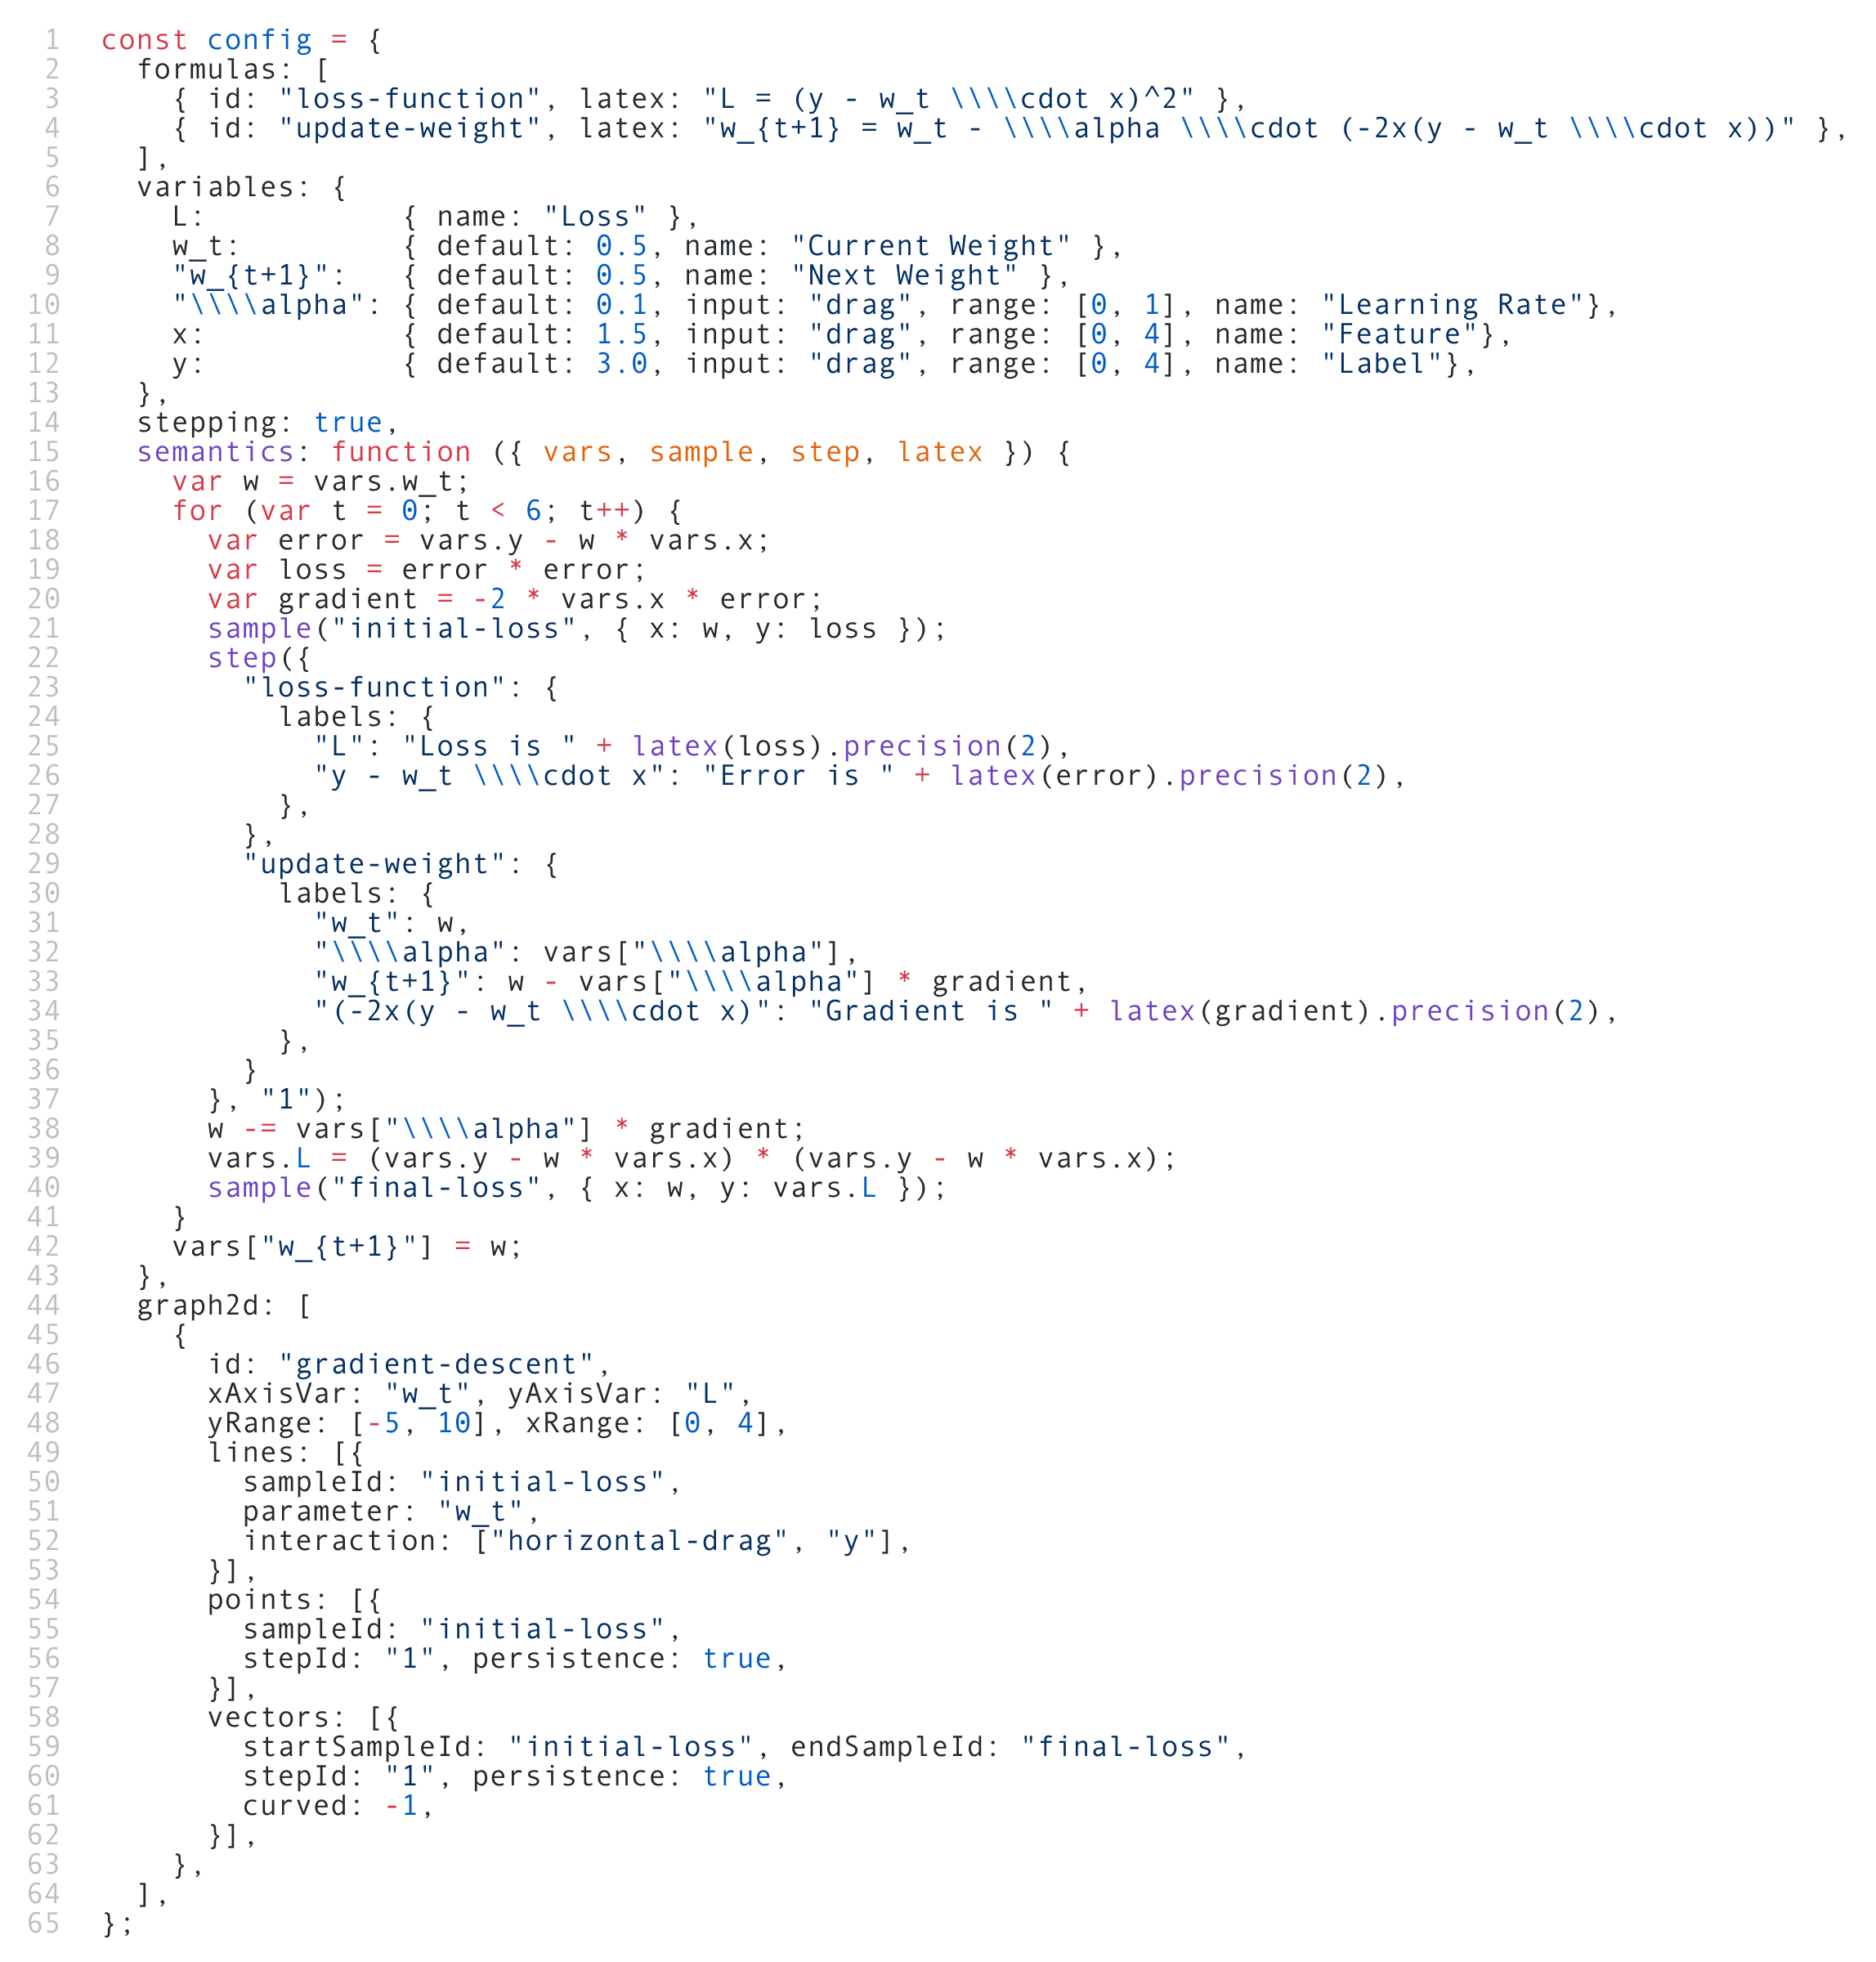
\includegraphics[width=\textwidth]{fig/gradient.png}
\captionof{figure}{Delta configuration for gradient descent walkthrough (Figure~\ref{fig:system}). \textmd{The specification declares two formulas, five interactive variables, and a semantics function that loops through training iterations, emitting \texttt{step()} calls with labels keyed by formula \texttt{id}.}}
\label{fig:gradient-config}
\end{minipage}

\clearpage

\section{Study 1 Details}

\subsubsection{Participant backgrounds}

Participants rated their comfort writing LaTeX formulas as a median of 4 on a 5-point Likert scale ($\sigma = 0.91$); 11 wrote LaTeX weekly, 5 monthly, and 3 less than monthly. They rated their comfort writing JavaScript as a median of 4 ($\sigma = 1.12$); 9 wrote JS weekly, 8 monthly, 1 daily, and 1 less than monthly. Regarding React experience, 6 had written substantial amounts of React in a professional context, 6 had written substantial amounts in personal or academic projects, and 7 had written small amounts in personal or academic projects. We refer to these participants by anonymized random double-digit numeric identifiers (e.g., P21, P48).

\subsubsection{Task time by order of interface assignment}
\label{sec:order-effect}

We observed a significant order effect on the magnitude of the time difference between conditions (Mann-Whitney $U = 88.0$, $p < .001$). Participants who used the baseline first showed a larger advantage for Delta (mean difference $= 8.9$ min) than those who used Delta first (mean difference $= 1.8$ min). This suggests that task familiarity compressed completion times in the second condition regardless of library. Critically, even within the more conservative subgroup that used Delta \textit{first}, Delta was still significantly faster (Wilcoxon $W = 6.0$, $p = .027$, $n = 10$), with 7 of 10 participants completing the task faster with Delta.

\subsubsection{Analysis of participant free-text responses}
\label{sec:free-text-analysis}

Participants' free-text responses revealed qualitative differences in \textit{where} each tool imposed cognitive load. We organize these findings using the Cognitive Dimensions of Notations framework~\cite{Blackwell2003-gv}, a widely adopted vocabulary for evaluating the usability of programming languages and notation systems. Three dimensions emerged most clearly.

\paragraph{Viscosity.} 
The most frequently cited baseline pain point was the effort required to make even a small change. Seven participants (P45, P55, P79, P80, P87, P88, P99) described the baseline as requiring coordinated edits across disconnected locations---state declarations, component props, and the LaTeX string (P55: ``making the small change to make m modifiable with a drag motion required changes in several parts of the code''). The \texttt{\textbackslash cssId\{\}} mechanism was a specific source of friction: seven participants (P11, P14, P20, P79, P87, P88, P99) reported confusion or errors matching CSS identifiers across component props and LaTeX strings (e.g., P88: ``I forgot to add the cssId on the LaTeX element `m'\,'').

\paragraph{Closeness of mapping.}
Four participants (P11, P20, P79, P88) independently described Delta's structure---formulas, variables, and semantics---in terms that closely mirror the library's API, without being prompted. P11 explained: ``there's the semantics of a formula, the looks of a formula [LaTeX], and then different components of the formula. [Delta] naturally gave in to this description.'' [Delta] had these components and only these that I need to change.'' That participants independently reconstructed the library's decomposition suggests it maps closely to how authors naturally reason about interactive formula authoring.

\paragraph{Visibility.}
Delta's configuration also improved \emph{visibility}---the ease with which required parts of the notation can be identified. Ten of 19 participants cited co-location as an advantage: P29 found it ``way faster to just look at the code and immediately see all the moving parts at a glance''; P21 praised ``clear partitions for variables, so could find and update easily''; and P80 described Delta as grouping ``the variables/components (labels, dragging functionality, displayed value) together in an intuitive way.'' By contrast, the baseline scattered relevant parts across disconnected locations (P79: ``a lot of moving components---in the html, use state, two types of wrappers'').

Two participants (P29, P14) preferred the baseline on suitability and language dimensions despite completing the task faster with Delta, citing familiarity with React idioms---pointing to a tension between task-specific efficiency and integration with existing workflows.

\clearpage

\section{Study 2 details}

\begin{minipage}{\columnwidth}
\centering
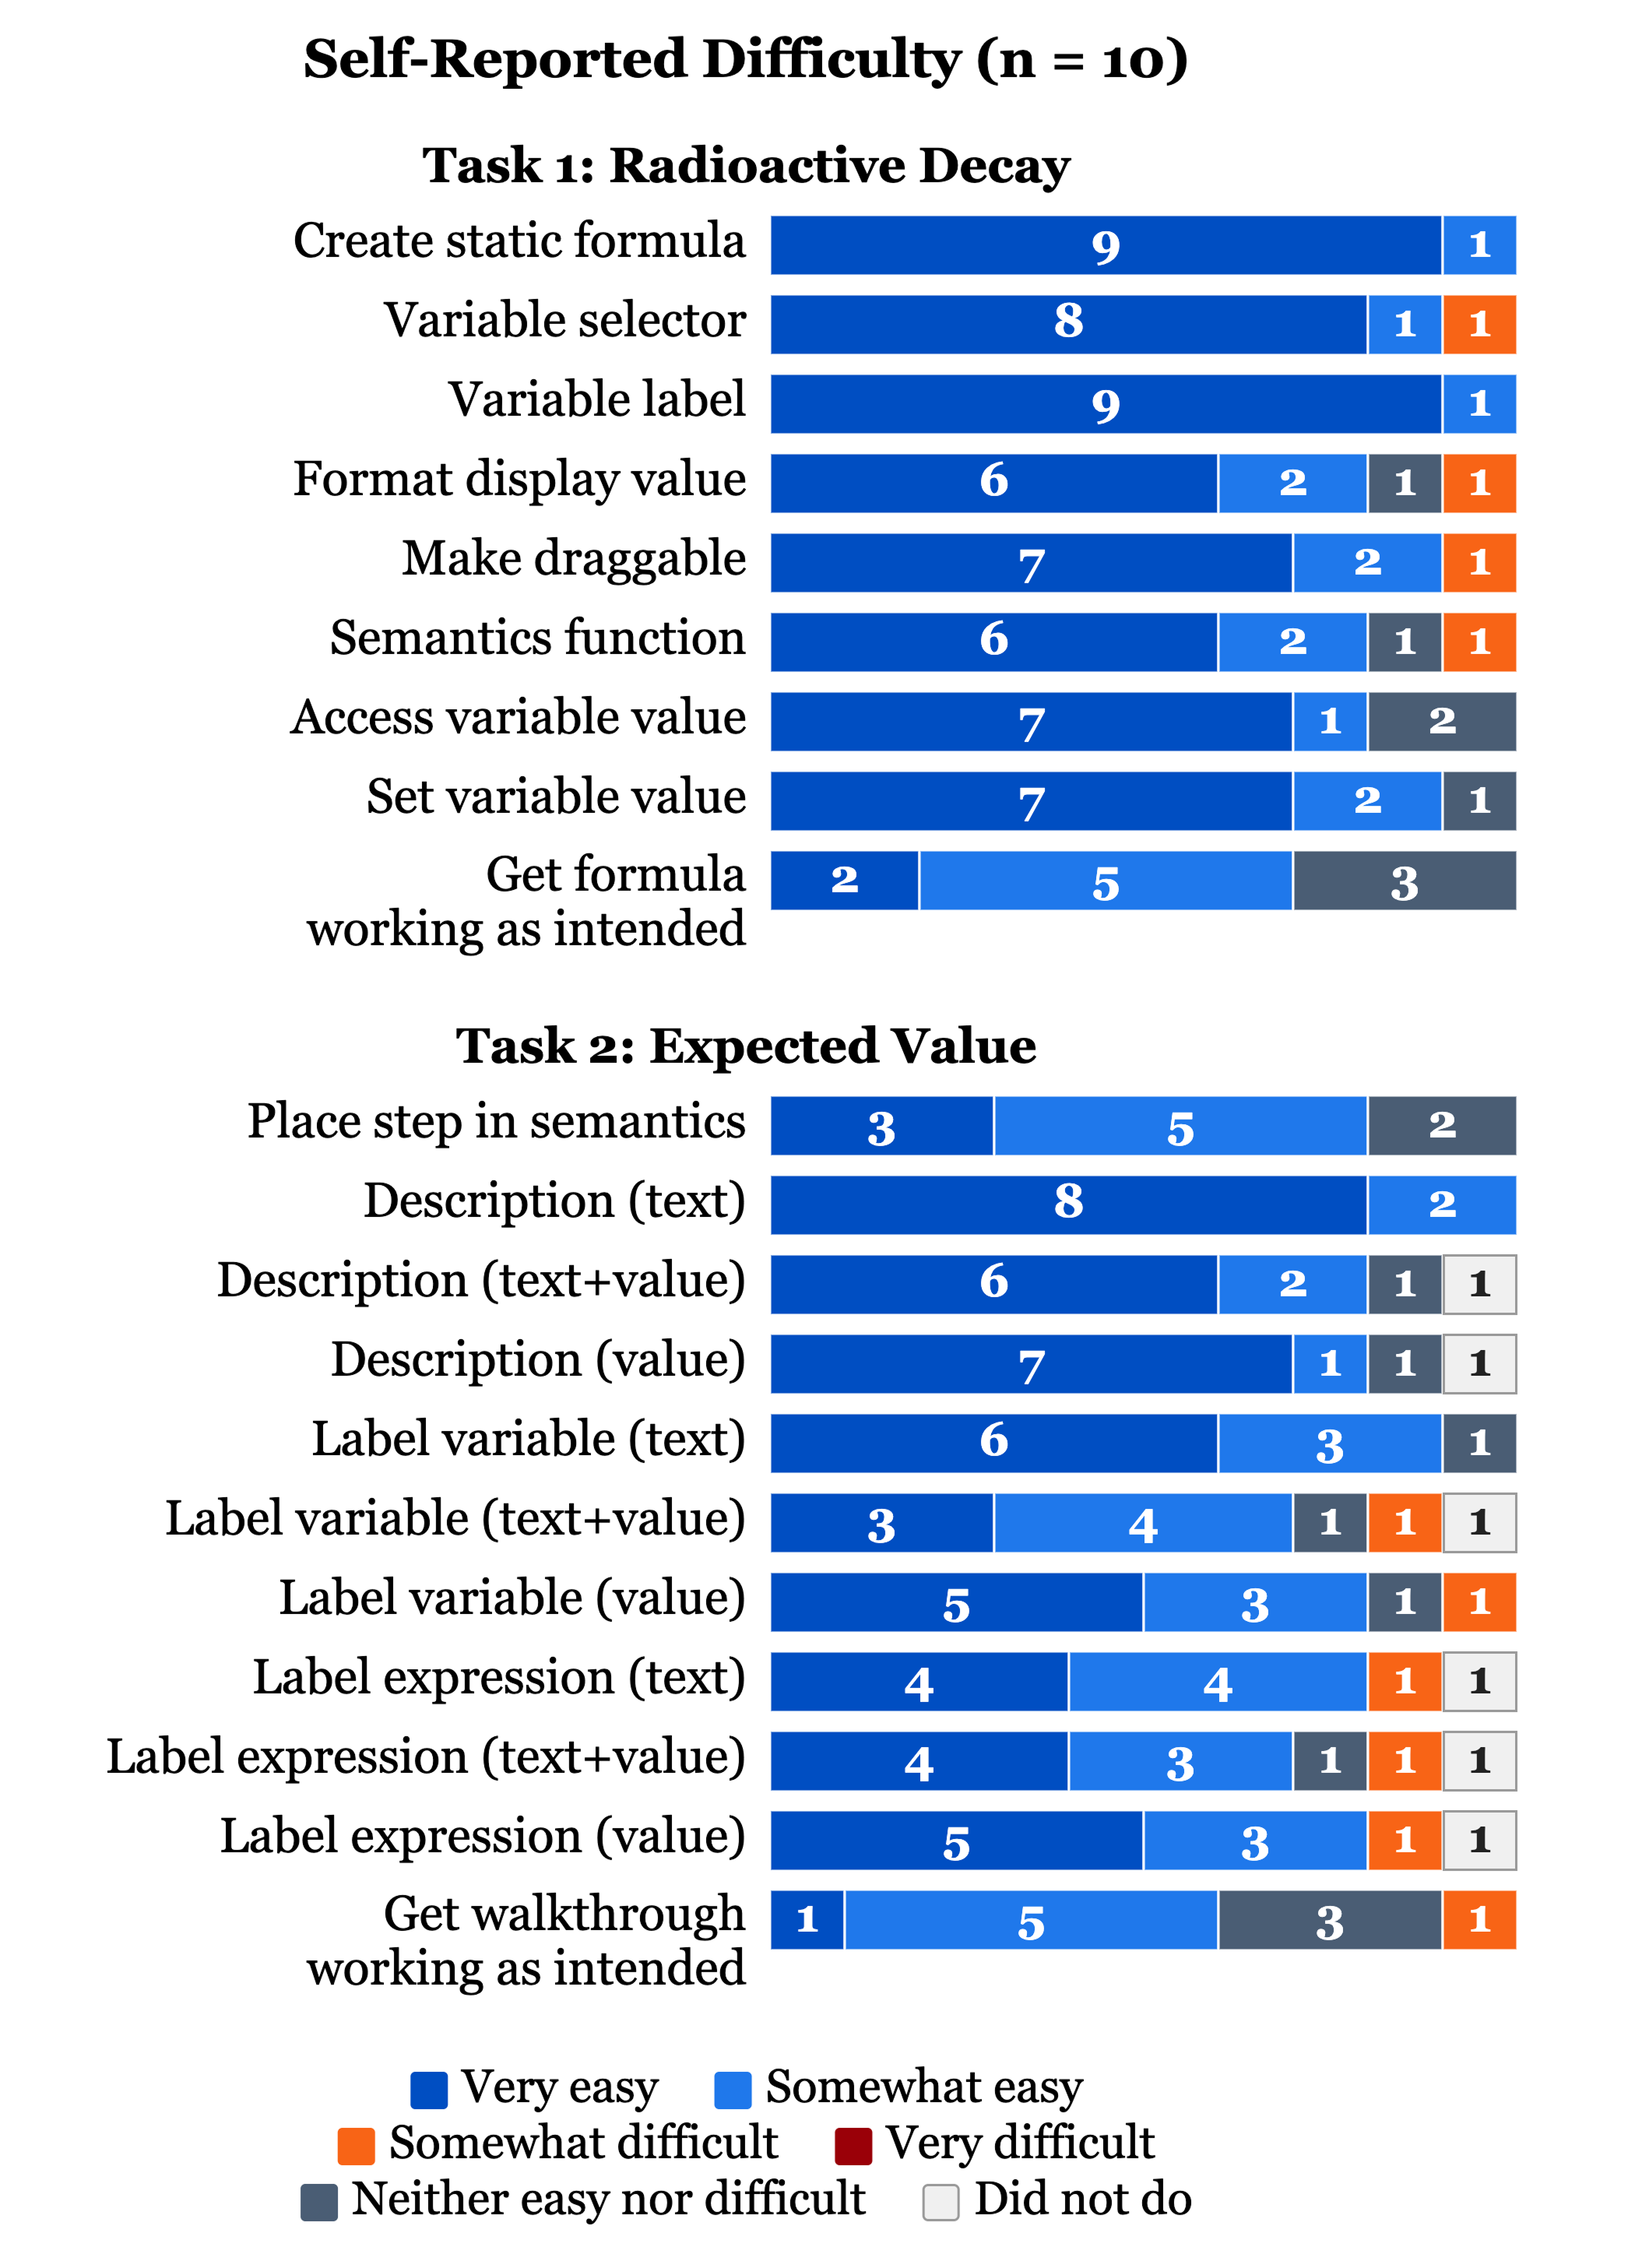
\includegraphics[width=\linewidth]{fig/difficulty.png}
\captionof{figure}{\textbf{Self-reported difficulty ratings.} Authors rated the difficulty of library features on a 5-point Likert scale ($n = 10$; some Task~2 features $n = 9$ due to ``did not do'' responses). \textmd{The distribution largely mirrors the intuitiveness ratings (Figure~\ref{fig:obs-intuitiveness}), with most features rated as easy or very easy.}}
\Description{Diverging stacked bar chart showing Likert-scale difficulty responses for both tasks side by side. The distribution is similar to the intuitiveness ratings, with most bars dominated by blue (very easy / somewhat easy).}
\label{fig:obs-difficulty}
\end{minipage}
% \vspace{-4ex}
\end{document}
